\documentclass[aspectratio=169,11pt]{beamer}

\usepackage[T1]{fontenc}
\usepackage{lmodern}
\usepackage{graphicx}
\usepackage{booktabs}
\usepackage{tikz}
\usepackage{pgfplots}
\pgfplotsset{compat=1.16}
\usetikzlibrary{positioning,arrows.meta,shapes.geometric,calc,fit,backgrounds}

% ---------- palette ----------
\definecolor{navy}{HTML}{111111}
\definecolor{amber}{HTML}{3A3A3A}
\definecolor{teal}{HTML}{7A7A7A}
\definecolor{coral}{HTML}{5A5A5A}
\definecolor{peri}{HTML}{9A9A9A}
\definecolor{paper}{HTML}{F0F0F0}
\definecolor{ink}{HTML}{1A1A1A}
\definecolor{cAmber}{HTML}{E09F1F}
\definecolor{cTeal}{HTML}{2A9D8F}
\definecolor{cCoral}{HTML}{E76F51}
\definecolor{cBlue}{HTML}{3F51B5}
\definecolor{mute}{HTML}{6E6E6E}

% ---------- beamer look ----------
\usetheme{default}
\usefonttheme{professionalfonts}
\setbeamertemplate{navigation symbols}{}
\setbeamercolor{normal text}{fg=ink,bg=white}
\setbeamercolor{structure}{fg=navy}
\setbeamercolor{frametitle}{fg=white,bg=navy}
\setbeamercolor{itemize item}{fg=amber}
\setbeamercolor{itemize subitem}{fg=amber}
\setbeamercolor{enumerate item}{fg=amber}
\setbeamercolor{block title}{fg=white,bg=navy}
\setbeamercolor{block body}{fg=ink,bg=paper}
\setbeamerfont{frametitle}{series=\bfseries,size=\Large}
\setbeamerfont{block title}{series=\bfseries,size=\normalsize}
\setbeamertemplate{itemize item}{\small$\blacktriangleright$}
\setbeamertemplate{blocks}[rounded][shadow=false]

\setbeamertemplate{frametitle}{%
  \nointerlineskip
  \begin{tikzpicture}[remember picture,overlay]
    \fill[navy] (current page.north west) rectangle ([yshift=-1.25cm]current page.north east);
    \node[anchor=center,text=white,font=\Large\bfseries] at ([yshift=-0.65cm]current page.north) {\insertframetitle};
  \end{tikzpicture}\vspace{0.6cm}%
}
\setbeamertemplate{footline}{%
  \hspace*{0.9cm}{\scriptsize\color{mute}DYNAMIC SCENE GRAPH \textbullet\ VIDOR \textbullet\ REVIEW 3}\hfill
  {\scriptsize\color{mute}\insertframenumber\,/\,\inserttotalframenumber}\hspace*{0.9cm}\vspace{0.35cm}}
\setbeamersize{text margin left=0.9cm,text margin right=0.9cm}

\newcommand{\stat}[3]{% value, label, colour
  \begin{tikzpicture}
    \node[fill=paper,rounded corners=6pt,minimum width=3.6cm,minimum height=2.3cm,align=center,inner sep=6pt]
      {{\Huge\bfseries\color{#3}#1}\\[3pt]{\small\color{mute}#2}};
  \end{tikzpicture}}

\title{Dynamic Scene Graph Generation from Video}
\subtitle{Review 3 \textbullet\ VidOR dataset}
\date{\today}

\begin{document}

% ======================= 1  TITLE =======================
\begin{frame}[plain]
  \begin{tikzpicture}[remember picture,overlay]
    \fill[black] (current page.south west) rectangle (current page.north east);
    \node[text=white!60!black,font=\bfseries\small,align=center] at ([yshift=-1.1cm]current page.north) {REVIEW 3 \ \textbullet\ \ VIDOR DATASET};
    \node[text=white,font=\fontsize{28}{32}\selectfont\bfseries,text width=12cm,align=center] at ([yshift=-3.0cm]current page.north)
      {Dynamic Scene Graph Generation from Video};
    \node[text=white!70!black,font=\normalsize,text width=10cm,align=center] at ([yshift=-4.75cm]current page.north)
      {Detect objects, track them through time, and predict how they relate --- frame by frame.};
    % horizontal scene graph
    \begin{scope}[shift={([yshift=-6.3cm]current page.north)}]
      \tikzset{g/.style={circle,draw=white,line width=1.3pt,fill=white!12!black,text=white,minimum size=1.15cm,font=\scriptsize\bfseries}}
      \node[g] (a) at (-4.8,0) {adult};
      \node[g] (b) at (-1.6,0) {baby};
      \node[g] (c) at (1.6,0) {table};
      \node[g] (d) at (4.8,0) {toy};
      \draw[white!70!black,thick] (a)--(b) node[midway,above,text=white!80!black,font=\scriptsize\itshape]{holds};
      \draw[white!70!black,thick] (b)--(c) node[midway,above,text=white!80!black,font=\scriptsize\itshape]{on};
      \draw[white!70!black,thick] (c)--(d) node[midway,above,text=white!80!black,font=\scriptsize\itshape]{beside};
    \end{scope}
    \node[draw=white,rounded corners=10pt,text=white,font=\bfseries\small,inner xsep=12pt,inner ysep=5pt] at ([yshift=-7.6cm]current page.north)
      {VidOR parts 1--8 trained \ \textbullet\ \ 78-class pipeline};
  \end{tikzpicture}
\end{frame}

% ======================= 2  PROBLEM =======================
\begin{frame}{A video is a story of who does what to whom}
  \centering
  \begin{columns}[T]
    \column{0.56\textwidth}
      \centering
      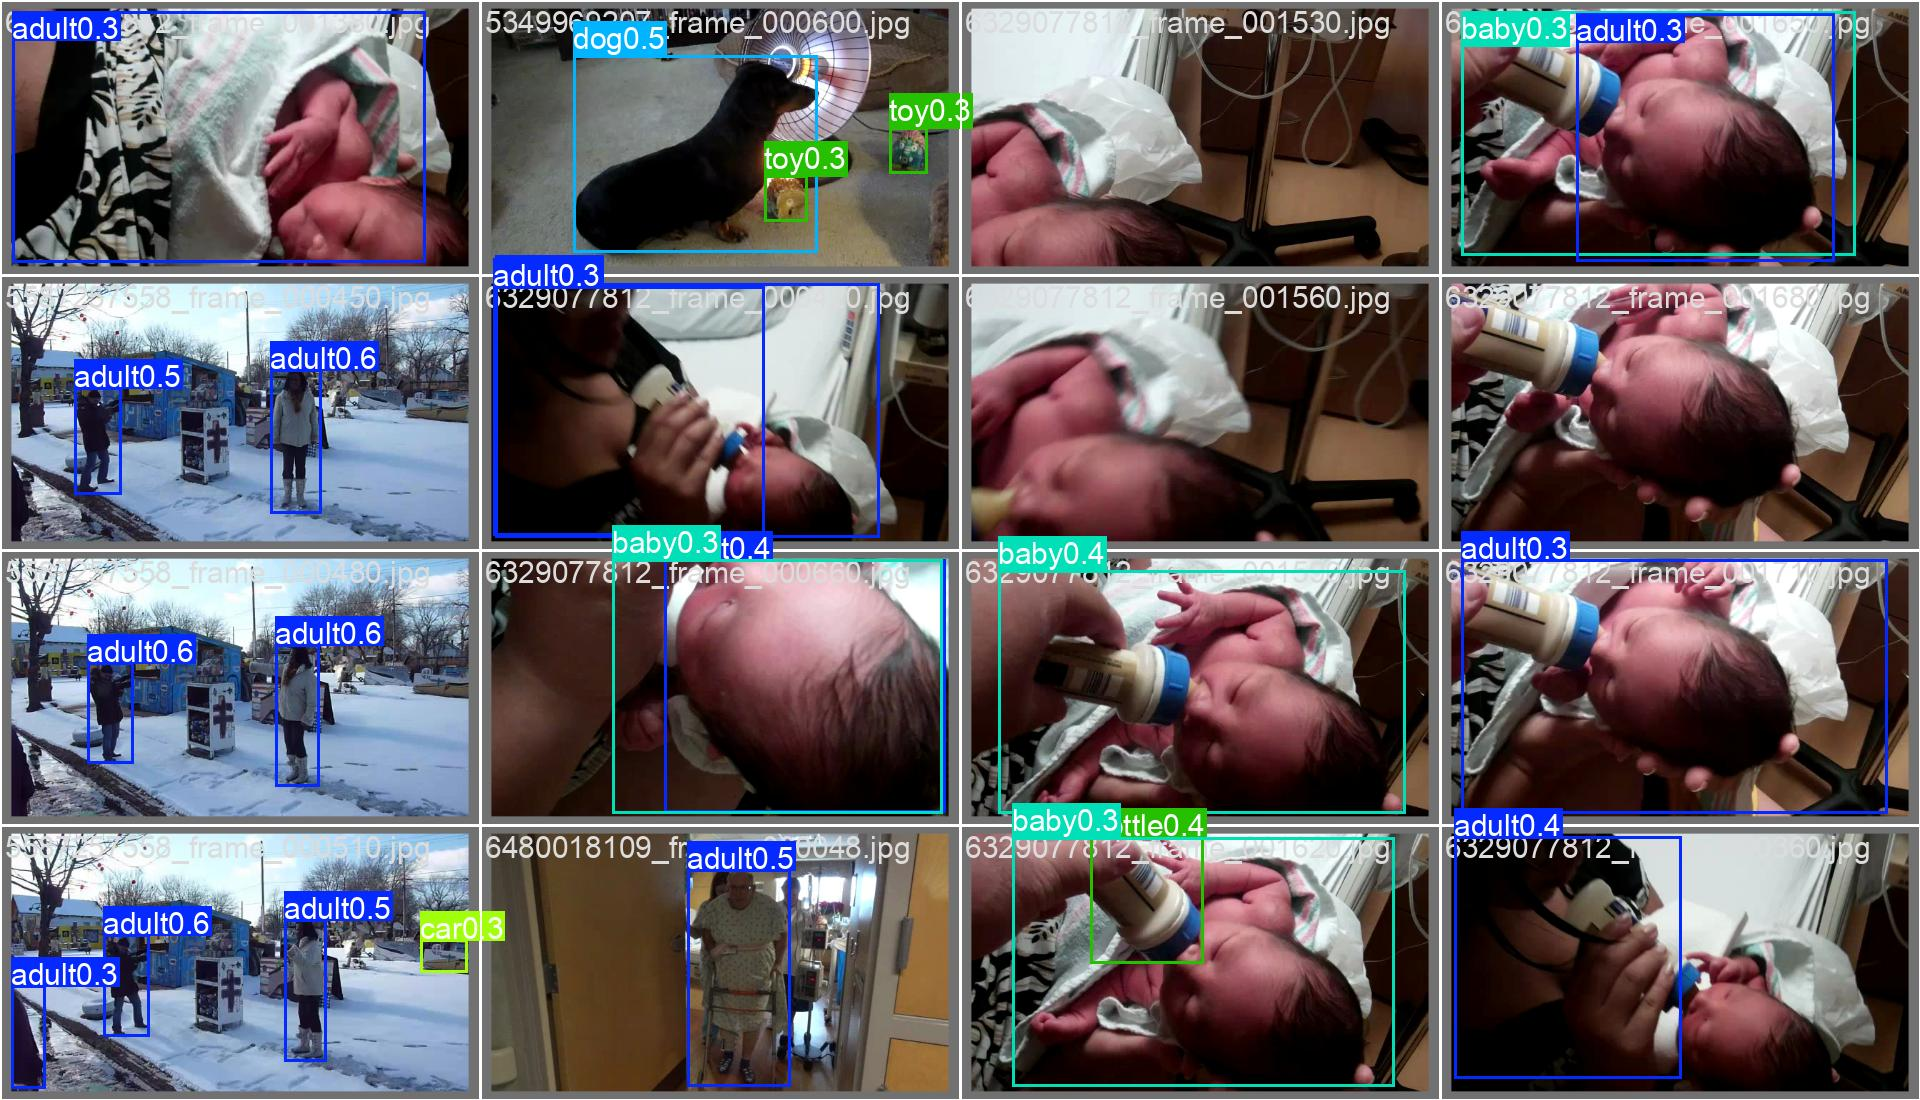
\includegraphics[width=\textwidth]{images/val_batch1_pred.jpg}\\[2pt]
      {\scriptsize\color{mute}\itshape Real validation frames with detector output (run 3)}
    \column{0.40\textwidth}
      \centering
      {\small\bfseries\color{mute} OUTPUT PER FRAME \textit{(illustrative)}}\\[6pt]
      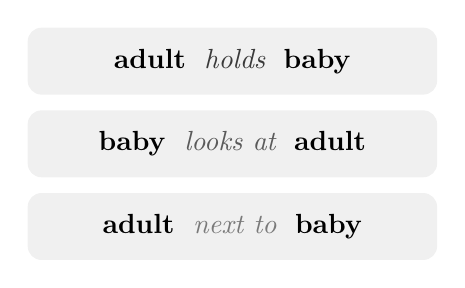
\begin{tikzpicture}
        \foreach \a/\r/\b/\c [count=\i from 0] in {adult/holds/baby/amber, baby/looks at/adult/coral, adult/next to/baby/teal}
          \node[fill=paper,rounded corners=5pt,minimum width=5.2cm,minimum height=0.85cm,anchor=north west,align=left,inner xsep=8pt]
            at (0,-\i*1.05) {\textbf{\a}\ \ {\color{\c}\itshape\r}\ \ \textbf{\b}};
      \end{tikzpicture}\\[10pt]
      {\small Doing this for every frame, with objects that keep their identity over time, is the task this project tackles.}
  \end{columns}
\end{frame}

% ======================= 3  STATIC VS DYNAMIC =======================
\begin{frame}{Per-frame graphs miss what changes over time}
  \centering
  \begin{columns}[T]
    \column{0.48\textwidth}
      \centering
      \begin{block}{Static (per frame)}
        \begin{itemize}\setlength\itemsep{2pt}
          \item Each frame labelled on its own
          \item No identity link between frames
          \item Relations flicker on and off
        \end{itemize}
      \end{block}
    \column{0.48\textwidth}
      \centering
      \begin{block}{Dynamic (this project)}
        \begin{itemize}\setlength\itemsep{2pt}
          \item Tracked objects keep one ID
          \item Relations have a start and an end
          \item Context from neighbouring frames
        \end{itemize}
      \end{block}
  \end{columns}
  \vspace{4pt}
  {\small\bfseries\color{mute} RELATIONS AS INTERVALS}\\[2pt]
  \begin{center}
  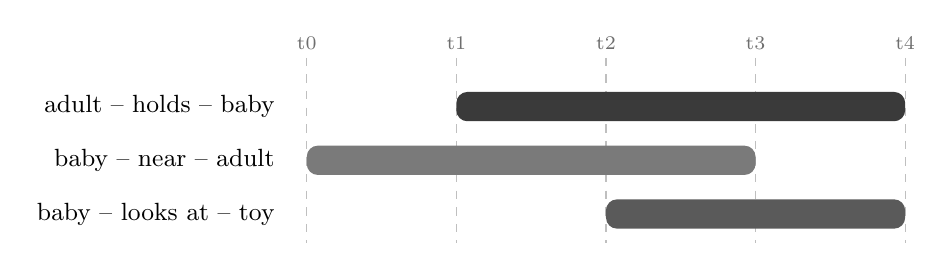
\begin{tikzpicture}[x=1.9cm,y=0.62cm]
    \foreach \x/\t in {0/t0,1/t1,2/t2,3/t3,4/t4}{
      \node[font=\scriptsize,text=mute] at (\x,0.8) {\t};
      \draw[dashed,gray!50] (\x,0.5) -- (\x,-3.3);}
    \node[anchor=east,font=\small] at (-0.15,-0.5) {adult -- holds -- baby};
    \node[anchor=east,font=\small] at (-0.15,-1.6) {baby -- near -- adult};
    \node[anchor=east,font=\small] at (-0.15,-2.7) {baby -- looks at -- toy};
    \fill[amber,rounded corners=4pt] (1,-0.8) rectangle (4,-0.2);
    \fill[teal,rounded corners=4pt]  (0,-1.9) rectangle (3,-1.3);
    \fill[coral,rounded corners=4pt] (2,-3.0) rectangle (4,-2.4);
  \end{tikzpicture}
  \end{center}
\end{frame}

% ======================= 4  DATASET =======================
\begin{frame}{VidOR comes in eight parts --- all eight are now trained}
  \centering
  \begin{columns}[T]
    \column{0.52\textwidth}
      \centering
      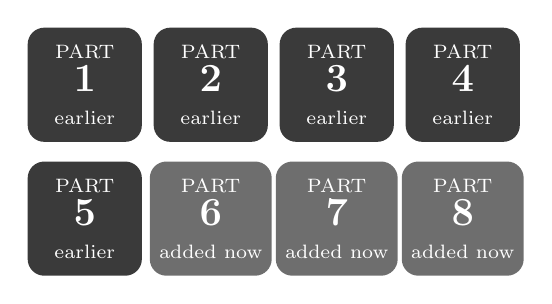
\begin{tikzpicture}
        \foreach \i in {1,...,5}{
          \pgfmathtruncatemacro{\col}{mod(\i-1,4)}
          \pgfmathtruncatemacro{\row}{int((\i-1)/4)}
          \node[fill=amber,rounded corners=6pt,minimum size=1.45cm,align=center,text=white] at (\col*1.6,-\row*1.7)
            {\scriptsize PART\\{\Large\bfseries\i}\\\scriptsize earlier};}
        \foreach \i in {6,...,8}{
          \pgfmathtruncatemacro{\col}{mod(\i-1,4)}
          \pgfmathtruncatemacro{\row}{int((\i-1)/4)}
          \node[fill=mute,rounded corners=6pt,minimum size=1.45cm,align=center,text=white] at (\col*1.6,-\row*1.7)
            {\scriptsize PART\\{\Large\bfseries\i}\\\scriptsize added now};}
      \end{tikzpicture}\\[6pt]
      {\scriptsize\color{mute} Dark = trained earlier \ \ Grey = added for this review}
    \column{0.44\textwidth}
      \centering
      \begin{tabular}{@{}rl@{}}
        {\LARGE\bfseries\color{amber}1 fps} & frame sampling\\[5pt]
        {\LARGE\bfseries\color{amber}60,588} & training frames\\[5pt]
        {\LARGE\bfseries\color{amber}3,594} & validation frames\\[5pt]
        {\LARGE\bfseries\color{amber}+750} & new videos (3 groups)
      \end{tabular}\\[8pt]
      {\scriptsize\color{mute}\itshape Training frames = 33,277 earlier + 27,311 new. Same validation set as before.}
  \end{columns}
\end{frame}

% ======================= 5  PIPELINE =======================
\begin{frame}{Eight stages from raw video to scene graph}
  \centering
  \begin{center}
  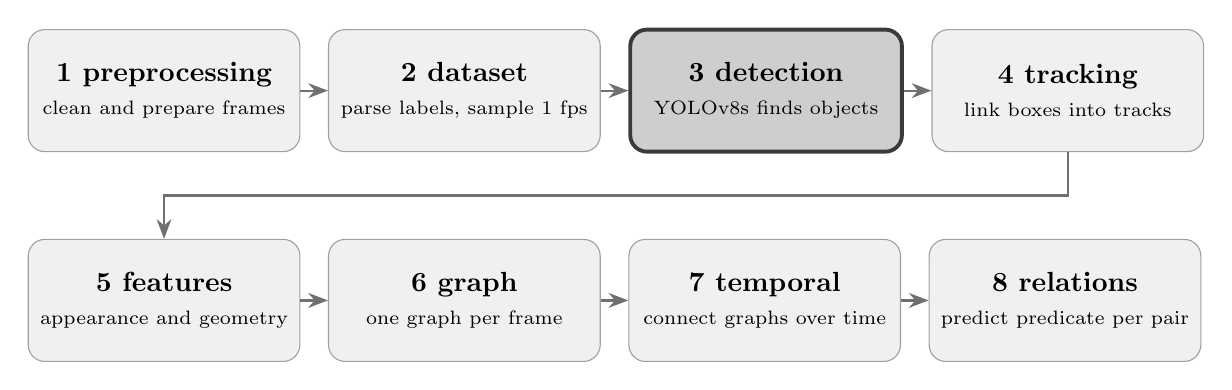
\begin{tikzpicture}[node distance=0.35cm,
      st/.style={rounded corners=6pt,fill=paper,draw=navy!40,minimum width=3.45cm,minimum height=1.55cm,align=center,inner sep=4pt},
      hot/.style={st,fill=amber!25,draw=amber,line width=1.4pt},
      ar/.style={-{Stealth[length=2.5mm]},thick,navy!60}]
    \node[st] (a) {{\bfseries 1 preprocessing}\\\scriptsize clean and prepare frames};
    \node[st,right=of a] (b) {{\bfseries 2 dataset}\\\scriptsize parse labels, sample 1 fps};
    \node[hot,right=of b] (c) {{\bfseries 3 detection}\\\scriptsize YOLOv8s finds objects};
    \node[st,right=of c] (d) {{\bfseries 4 tracking}\\\scriptsize link boxes into tracks};
    \node[st,below=1.1cm of a] (e) {{\bfseries 5 features}\\\scriptsize appearance and geometry};
    \node[st,right=of e] (f) {{\bfseries 6 graph}\\\scriptsize one graph per frame};
    \node[st,right=of f] (g) {{\bfseries 7 temporal}\\\scriptsize connect graphs over time};
    \node[st,right=of g] (h) {{\bfseries 8 relations}\\\scriptsize predict predicate per pair};
    \draw[ar] (a)--(b); \draw[ar] (b)--(c); \draw[ar] (c)--(d);
    \draw[ar] (d.south) |- ++(0,-0.55) -| (e.north);
    \draw[ar] (e)--(f); \draw[ar] (f)--(g); \draw[ar] (g)--(h);
  \end{tikzpicture}
  \end{center}
  {\small\bfseries\color{amber} Trained and evaluated: detection, the relation model and the temporal LSTM/GRU models.} {\small Later stages consume the detector's boxes, so detector quality sets the ceiling.}
\end{frame}

% ======================= 6  EXPORT =======================
\begin{frame}{What the dataset export contains}
  \centering
  \vspace{0.2cm}
  \begin{tabular}{@{}p{5.6cm}p{7.6cm}@{}}
    \toprule
    \textbf{Folder / file} & \textbf{Contents}\\
    \midrule
    \texttt{annotations} & VidOR labels for train and val\\
    \texttt{videos} & source clips\\
    \texttt{yolo\_format} & frames and boxes in YOLO layout\\
    \texttt{tracks} & per-video object tracks\\
    \texttt{features} & extracted object features\\
    \texttt{relation\_dataset} & object-pair relation samples\\
    \texttt{relation\_dataset\_corrected} & revised relation samples\\
    \texttt{dataset\_manifest.json} & parts, fps and counts\\
    \bottomrule
  \end{tabular}
\end{frame}

% ======================= 7  DETECTOR =======================
\begin{frame}{YOLOv8s: three Colab runs, then a fine-tune on all parts}
  \centering
  \begin{columns}[T]
    \column{0.48\textwidth}
      \centering
      \begin{tabular}{@{}ll@{}}
        \toprule
        Base model   & \textbf{yolov8s.pt}, pretrained\\
        Input size   & \textbf{640 px}\\
        Epochs       & \textbf{10} per run, \textbf{3} fine-tune\\
        Optimizer    & auto, lr0 = 0.01\\
        Augmentation & mosaic, flip 0.5, HSV\\
        Hardware     & Colab GPU, then M3 Pro Mac\\
        \bottomrule
      \end{tabular}
    \column{0.48\textwidth}
      \centering
      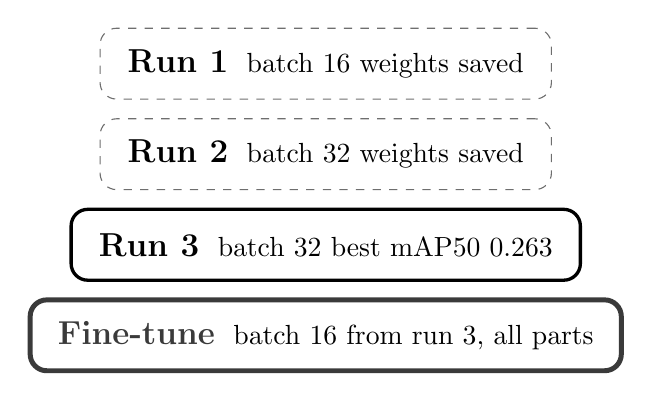
\begin{tikzpicture}
        \node[draw=mute,dashed,rounded corners=6pt,minimum width=5.6cm,minimum height=0.9cm,align=left,inner xsep=10pt] at (0,0)
          {{\large\bfseries Run 1}\ \ batch 16 \hfill weights saved};
        \node[draw=mute,dashed,rounded corners=6pt,minimum width=5.6cm,minimum height=0.9cm,align=left,inner xsep=10pt] at (0,-1.15)
          {{\large\bfseries Run 2}\ \ batch 32 \hfill weights saved};
        \node[draw=black,line width=1.2pt,rounded corners=6pt,minimum width=5.6cm,minimum height=0.9cm,align=left,inner xsep=10pt] at (0,-2.3)
          {{\large\bfseries Run 3}\ \ batch 32 \hfill best mAP50 0.263};
        \node[draw=amber,line width=1.8pt,rounded corners=6pt,minimum width=5.6cm,minimum height=0.9cm,align=left,inner xsep=10pt] at (0,-3.45)
          {{\large\bfseries\color{amber}Fine-tune}\ \ batch 16 \hfill from run 3, all parts};
      \end{tikzpicture}
  \end{columns}
\end{frame}

% ======================= 8  CHARTS =======================
\begin{frame}{mAP stalls near 0.25 as validation loss stays flat}
  \centering
  \begin{columns}[T]
    \column{0.49\textwidth}
      \centering
      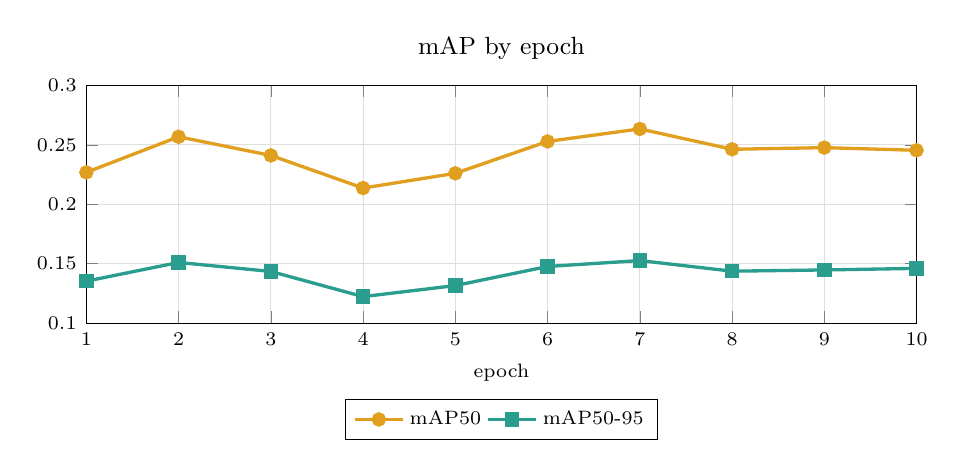
\begin{tikzpicture}
        \begin{axis}[width=\textwidth,height=4.6cm,title={\small mAP by epoch},xlabel={\scriptsize epoch},
          xmin=1,xmax=10,xtick={1,...,10},ymin=0.1,ymax=0.3,tick label style={font=\scriptsize},
          legend style={font=\scriptsize,at={(0.5,-0.32)},anchor=north,legend columns=2},grid=major,grid style={gray!25}]
          \addplot[color=cAmber,very thick,mark=*] coordinates {(1,0.22684)(2,0.25678)(3,0.24108)(4,0.21363)(5,0.22603)(6,0.25286)(7,0.26339)(8,0.24626)(9,0.24764)(10,0.2454)};
          \addlegendentry{mAP50}
          \addplot[color=cTeal,very thick,mark=square*] coordinates {(1,0.13529)(2,0.15102)(3,0.14345)(4,0.12227)(5,0.13157)(6,0.14764)(7,0.1526)(8,0.14368)(9,0.14472)(10,0.14602)};
          \addlegendentry{mAP50-95}
        \end{axis}
      \end{tikzpicture}
    \column{0.49\textwidth}
      \centering
      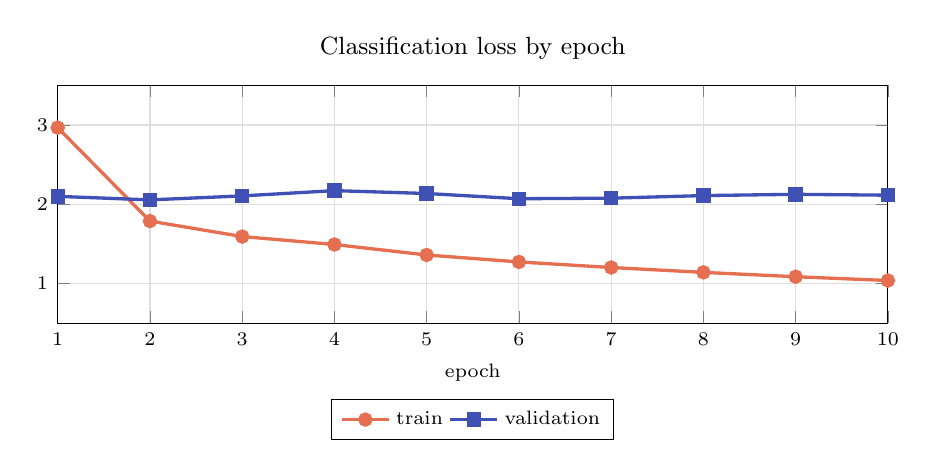
\begin{tikzpicture}
        \begin{axis}[width=\textwidth,height=4.6cm,title={\small Classification loss by epoch},xlabel={\scriptsize epoch},
          xmin=1,xmax=10,xtick={1,...,10},ymin=0.5,ymax=3.5,tick label style={font=\scriptsize},
          legend style={font=\scriptsize,at={(0.5,-0.32)},anchor=north,legend columns=2},grid=major,grid style={gray!25}]
          \addplot[color=cCoral,very thick,mark=*] coordinates {(1,2.96703)(2,1.78755)(3,1.5923)(4,1.49179)(5,1.35952)(6,1.272)(7,1.20149)(8,1.14002)(9,1.08518)(10,1.03725)};
          \addlegendentry{train}
          \addplot[color=cBlue,very thick,mark=square*] coordinates {(1,2.09962)(2,2.05509)(3,2.10536)(4,2.17195)(5,2.13572)(6,2.06972)(7,2.0767)(8,2.10949)(9,2.12532)(10,2.1144)};
          \addlegendentry{validation}
        \end{axis}
      \end{tikzpicture}
  \end{columns}
  \vspace{4pt}
  {\footnotesize Training loss keeps falling while validation loss stays near 2.1 --- a sign of over-fitting. Full run: 10 epochs, about 79 minutes on one Colab GPU.}
\end{frame}

% ======================= 9  STATS + PR =======================
\begin{frame}{Peak 0.263 mAP50 at epoch 7}
  \centering
  \begin{columns}[T]
    \column{0.46\textwidth}
      \centering
      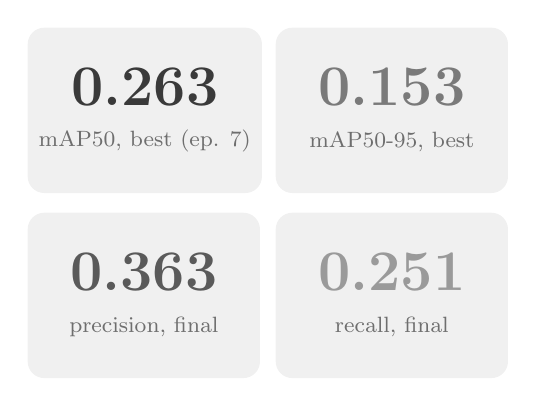
\begin{tikzpicture}
        \foreach \v/\l/\c/\x/\y in {0.263/{mAP50, best (ep. 7)}/amber/0/0, 0.153/{mAP50-95, best}/teal/3.15/0, 0.363/{precision, final}/coral/0/-2.35, 0.251/{recall, final}/peri/3.15/-2.35}
          \node[fill=paper,rounded corners=6pt,minimum width=2.95cm,minimum height=2.1cm,align=center,inner sep=4pt,anchor=north west] at (\x,\y)
            {{\huge\bfseries\color{\c}\v}\\[3pt]{\footnotesize\color{mute}\l}};
      \end{tikzpicture}
    \column{0.50\textwidth}
      \centering
      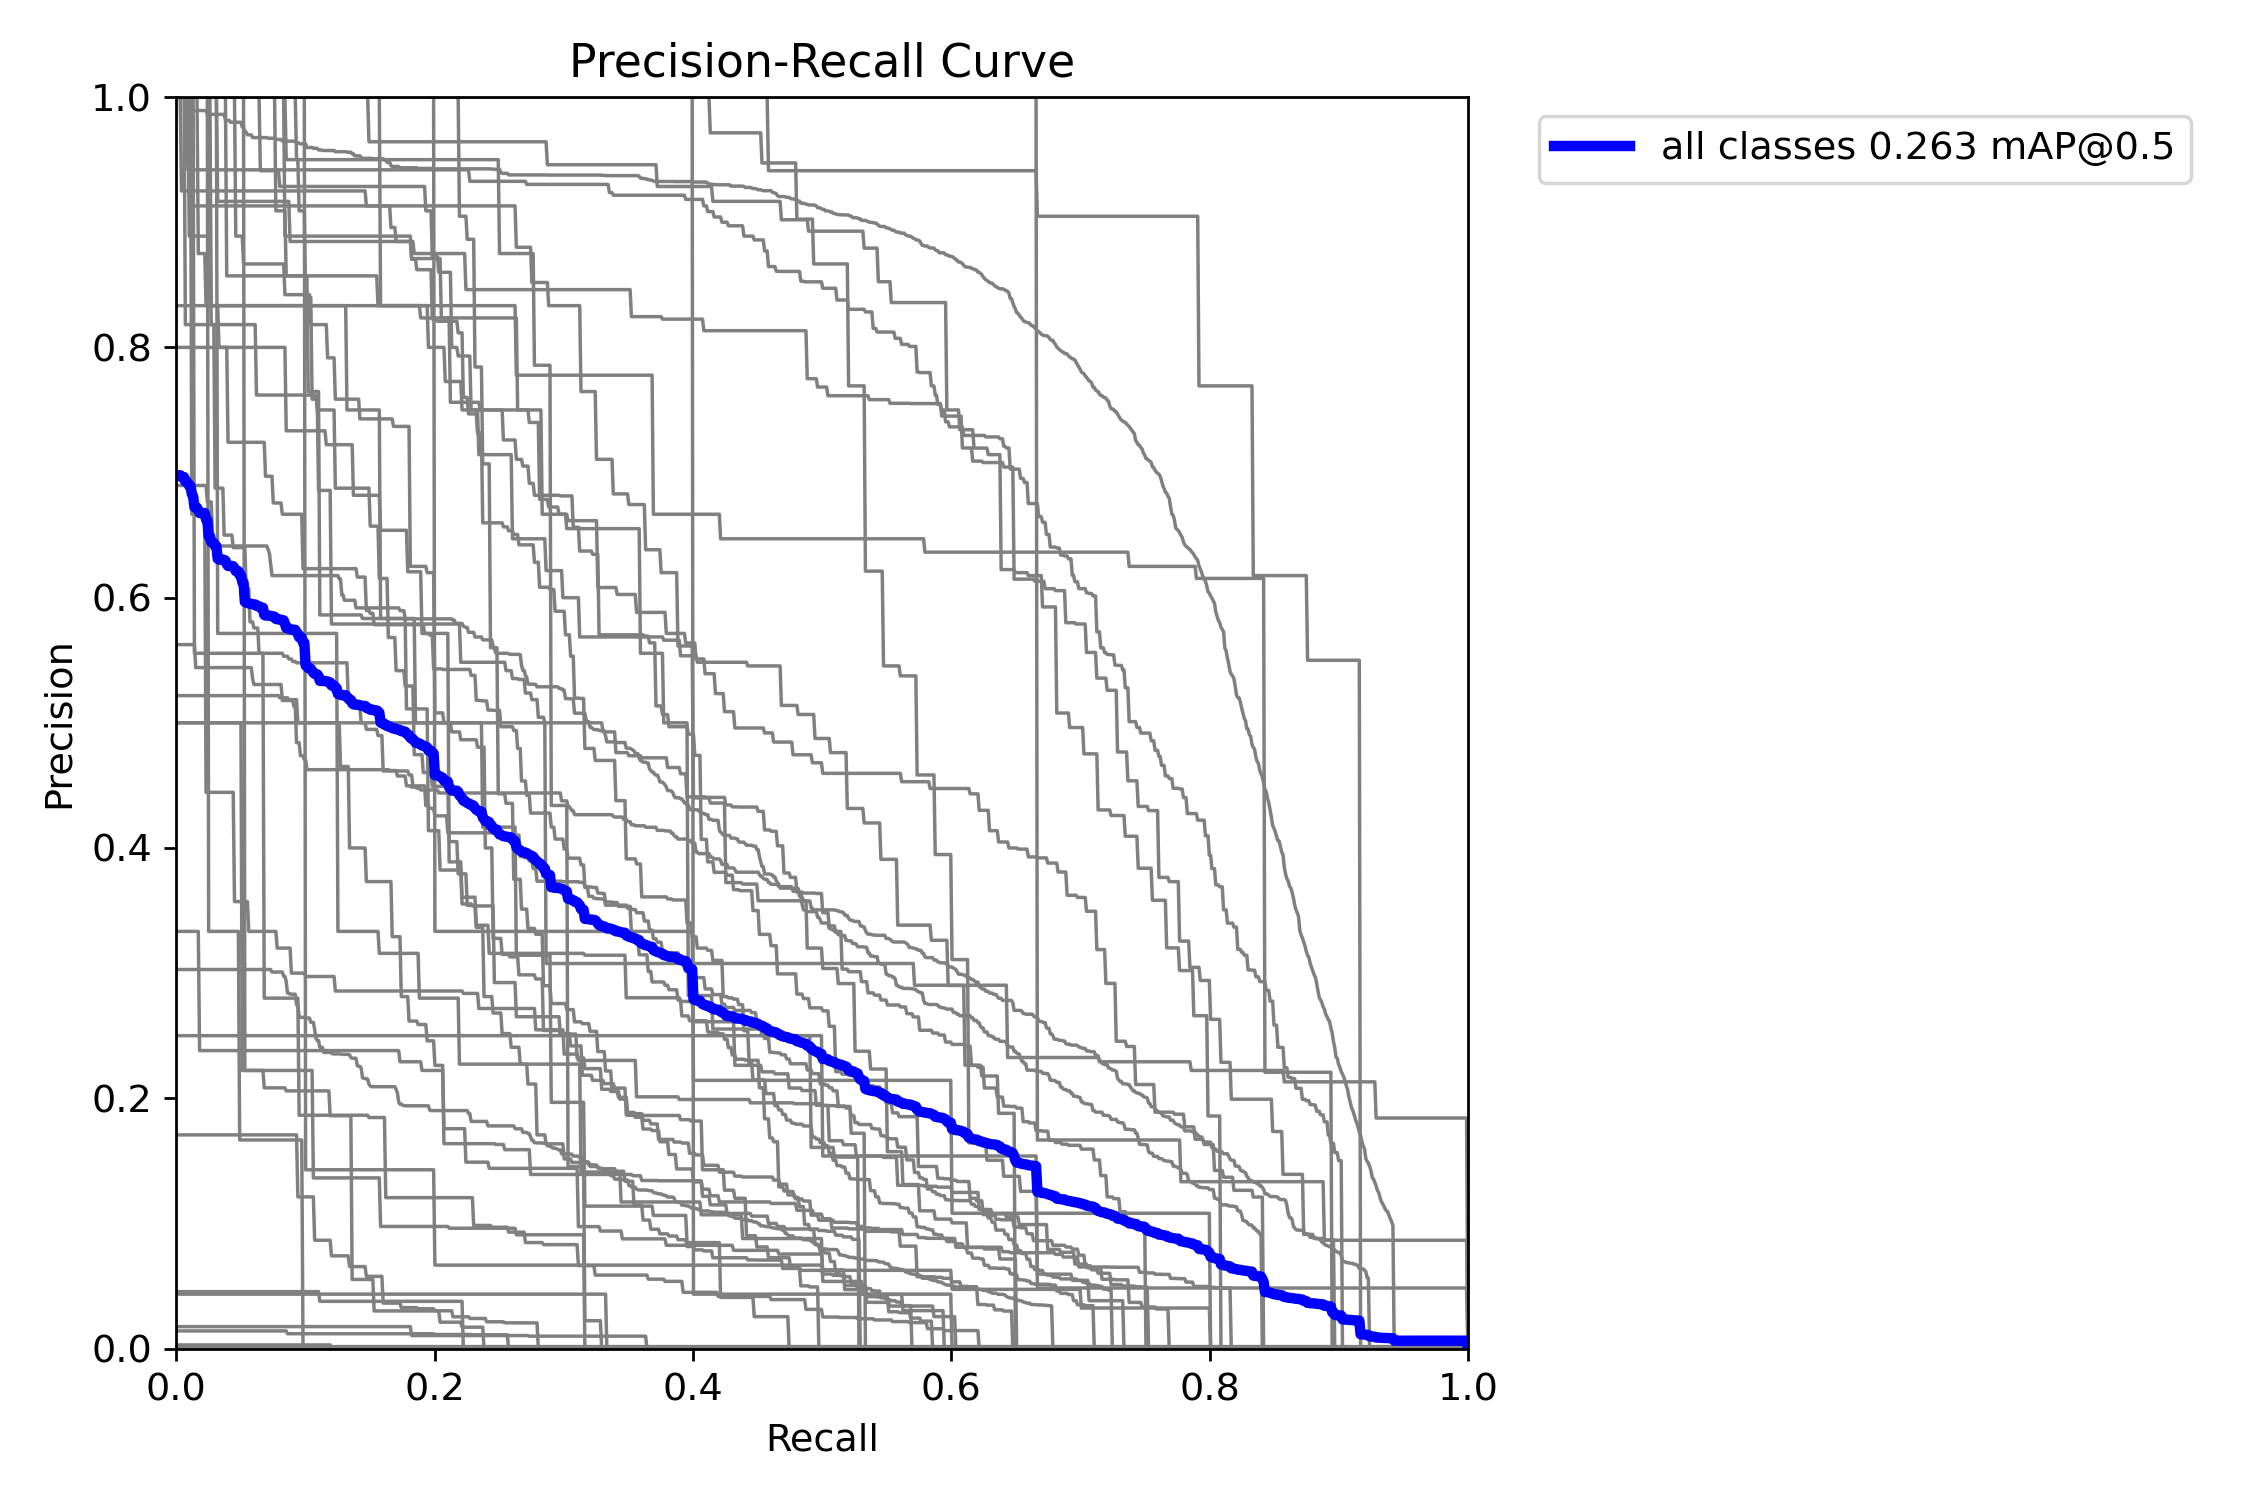
\includegraphics[width=\textwidth]{images/BoxPR_curve.png}\\[-2pt]
      {\scriptsize\color{mute} Precision--recall: all classes (blue) and each class (grey).}
  \end{columns}
\end{frame}

% ======================= FINE-TUNE RESULTS =======================
\begin{frame}[t]{Fine-tune on all parts: detector results}
  \centering\vspace{0.3cm}
  \begin{columns}[T]
    \column{0.44\textwidth}
      \centering
      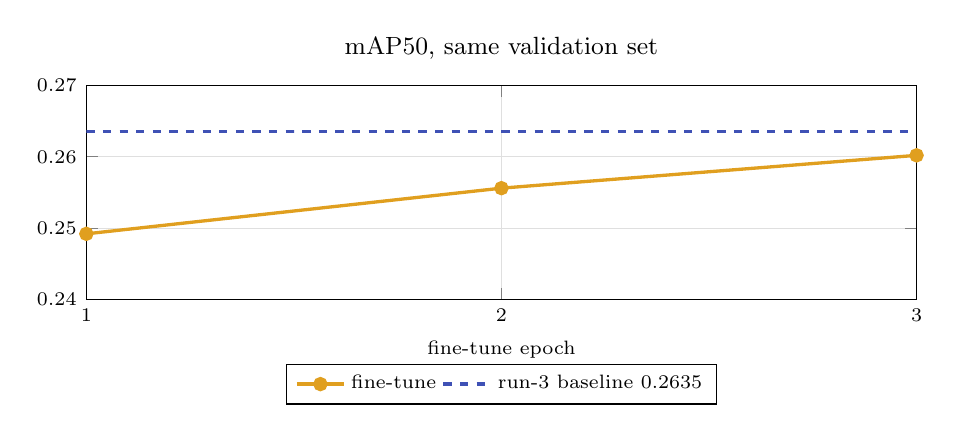
\begin{tikzpicture}
        \begin{axis}[width=\textwidth,height=4.3cm,title={\small mAP50, same validation set},xlabel={\scriptsize fine-tune epoch},
          xmin=1,xmax=3,xtick={1,2,3},ymin=0.24,ymax=0.27,ytick={0.24,0.25,0.26,0.27},tick label style={font=\scriptsize},
          legend style={font=\scriptsize,at={(0.5,-0.3)},anchor=north,legend columns=2},grid=major,grid style={gray!25}]
          \addplot[color=cAmber,very thick,mark=*] coordinates {(1,0.2492)(2,0.2556)(3,0.2602)};
          \addlegendentry{fine-tune}
          \addplot[color=cBlue,very thick,dashed,domain=1:3] {0.2635};
          \addlegendentry{run-3 baseline 0.2635}
        \end{axis}
      \end{tikzpicture}
    \column{0.54\textwidth}
      \centering\scriptsize\setlength{\tabcolsep}{3pt}
      \begin{tabular}{lcccc}
        \toprule
        & P & R & mAP50 & mAP50-95\\
        \midrule
        Baseline (run 3) & 0.381 & 0.285 & 0.2635 & 0.1526\\
        Epoch 1 & 0.410 & 0.235 & 0.2492 & 0.1471\\
        Epoch 2 & 0.407 & 0.272 & 0.2556 & 0.1508\\
        \textbf{Epoch 3} & \textbf{0.331} & \textbf{0.303} & \textbf{0.2602} & \textbf{0.1548}\\
        \bottomrule
      \end{tabular}
  \end{columns}
  \vspace{2pt}
  {\footnotesize 27,311 new frames did not raise mAP50 (0.2635 $\rightarrow$ 0.2602); recall rose and precision fell, mAP50-95 is slightly higher. Validation classification loss improved from about 2.1 to 1.96. Each epoch took about 76 minutes on an M3 Pro.}
\end{frame}

% ======================= FINE-TUNE GRAPHS =======================
\begin{frame}{Fine-tune training graphs}
  \centering
  \begin{columns}[T]
    \column{0.58\textwidth}
      \centering
      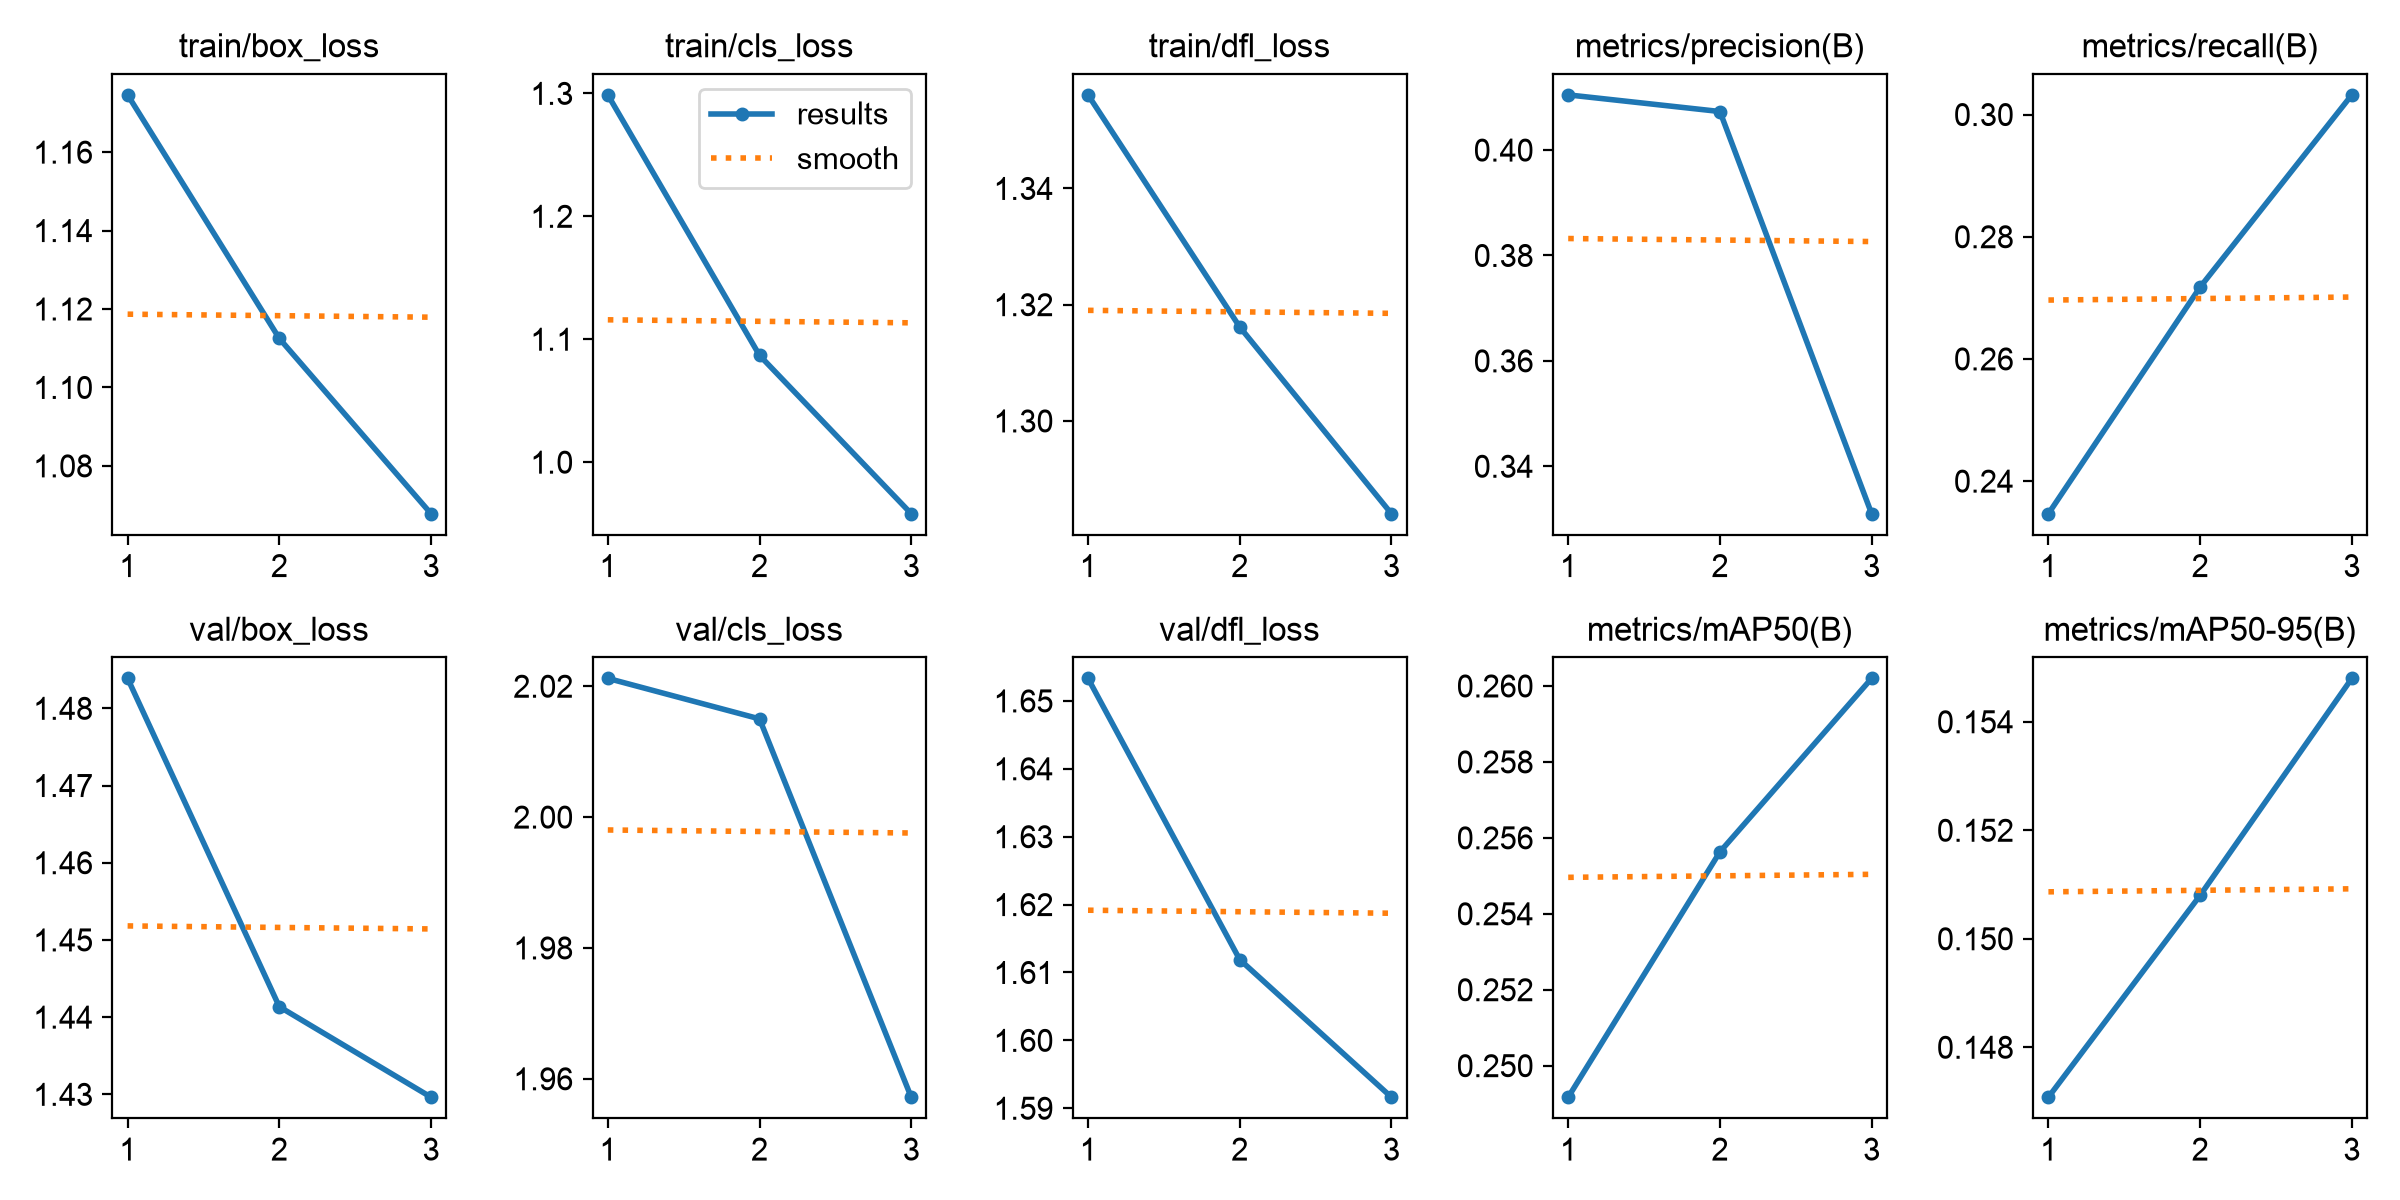
\includegraphics[width=\textwidth]{images/finetune_results.png}\\[-2pt]
      {\scriptsize\color{mute} Losses, precision, recall and mAP over the 3 fine-tune epochs.}
    \column{0.38\textwidth}
      \centering
      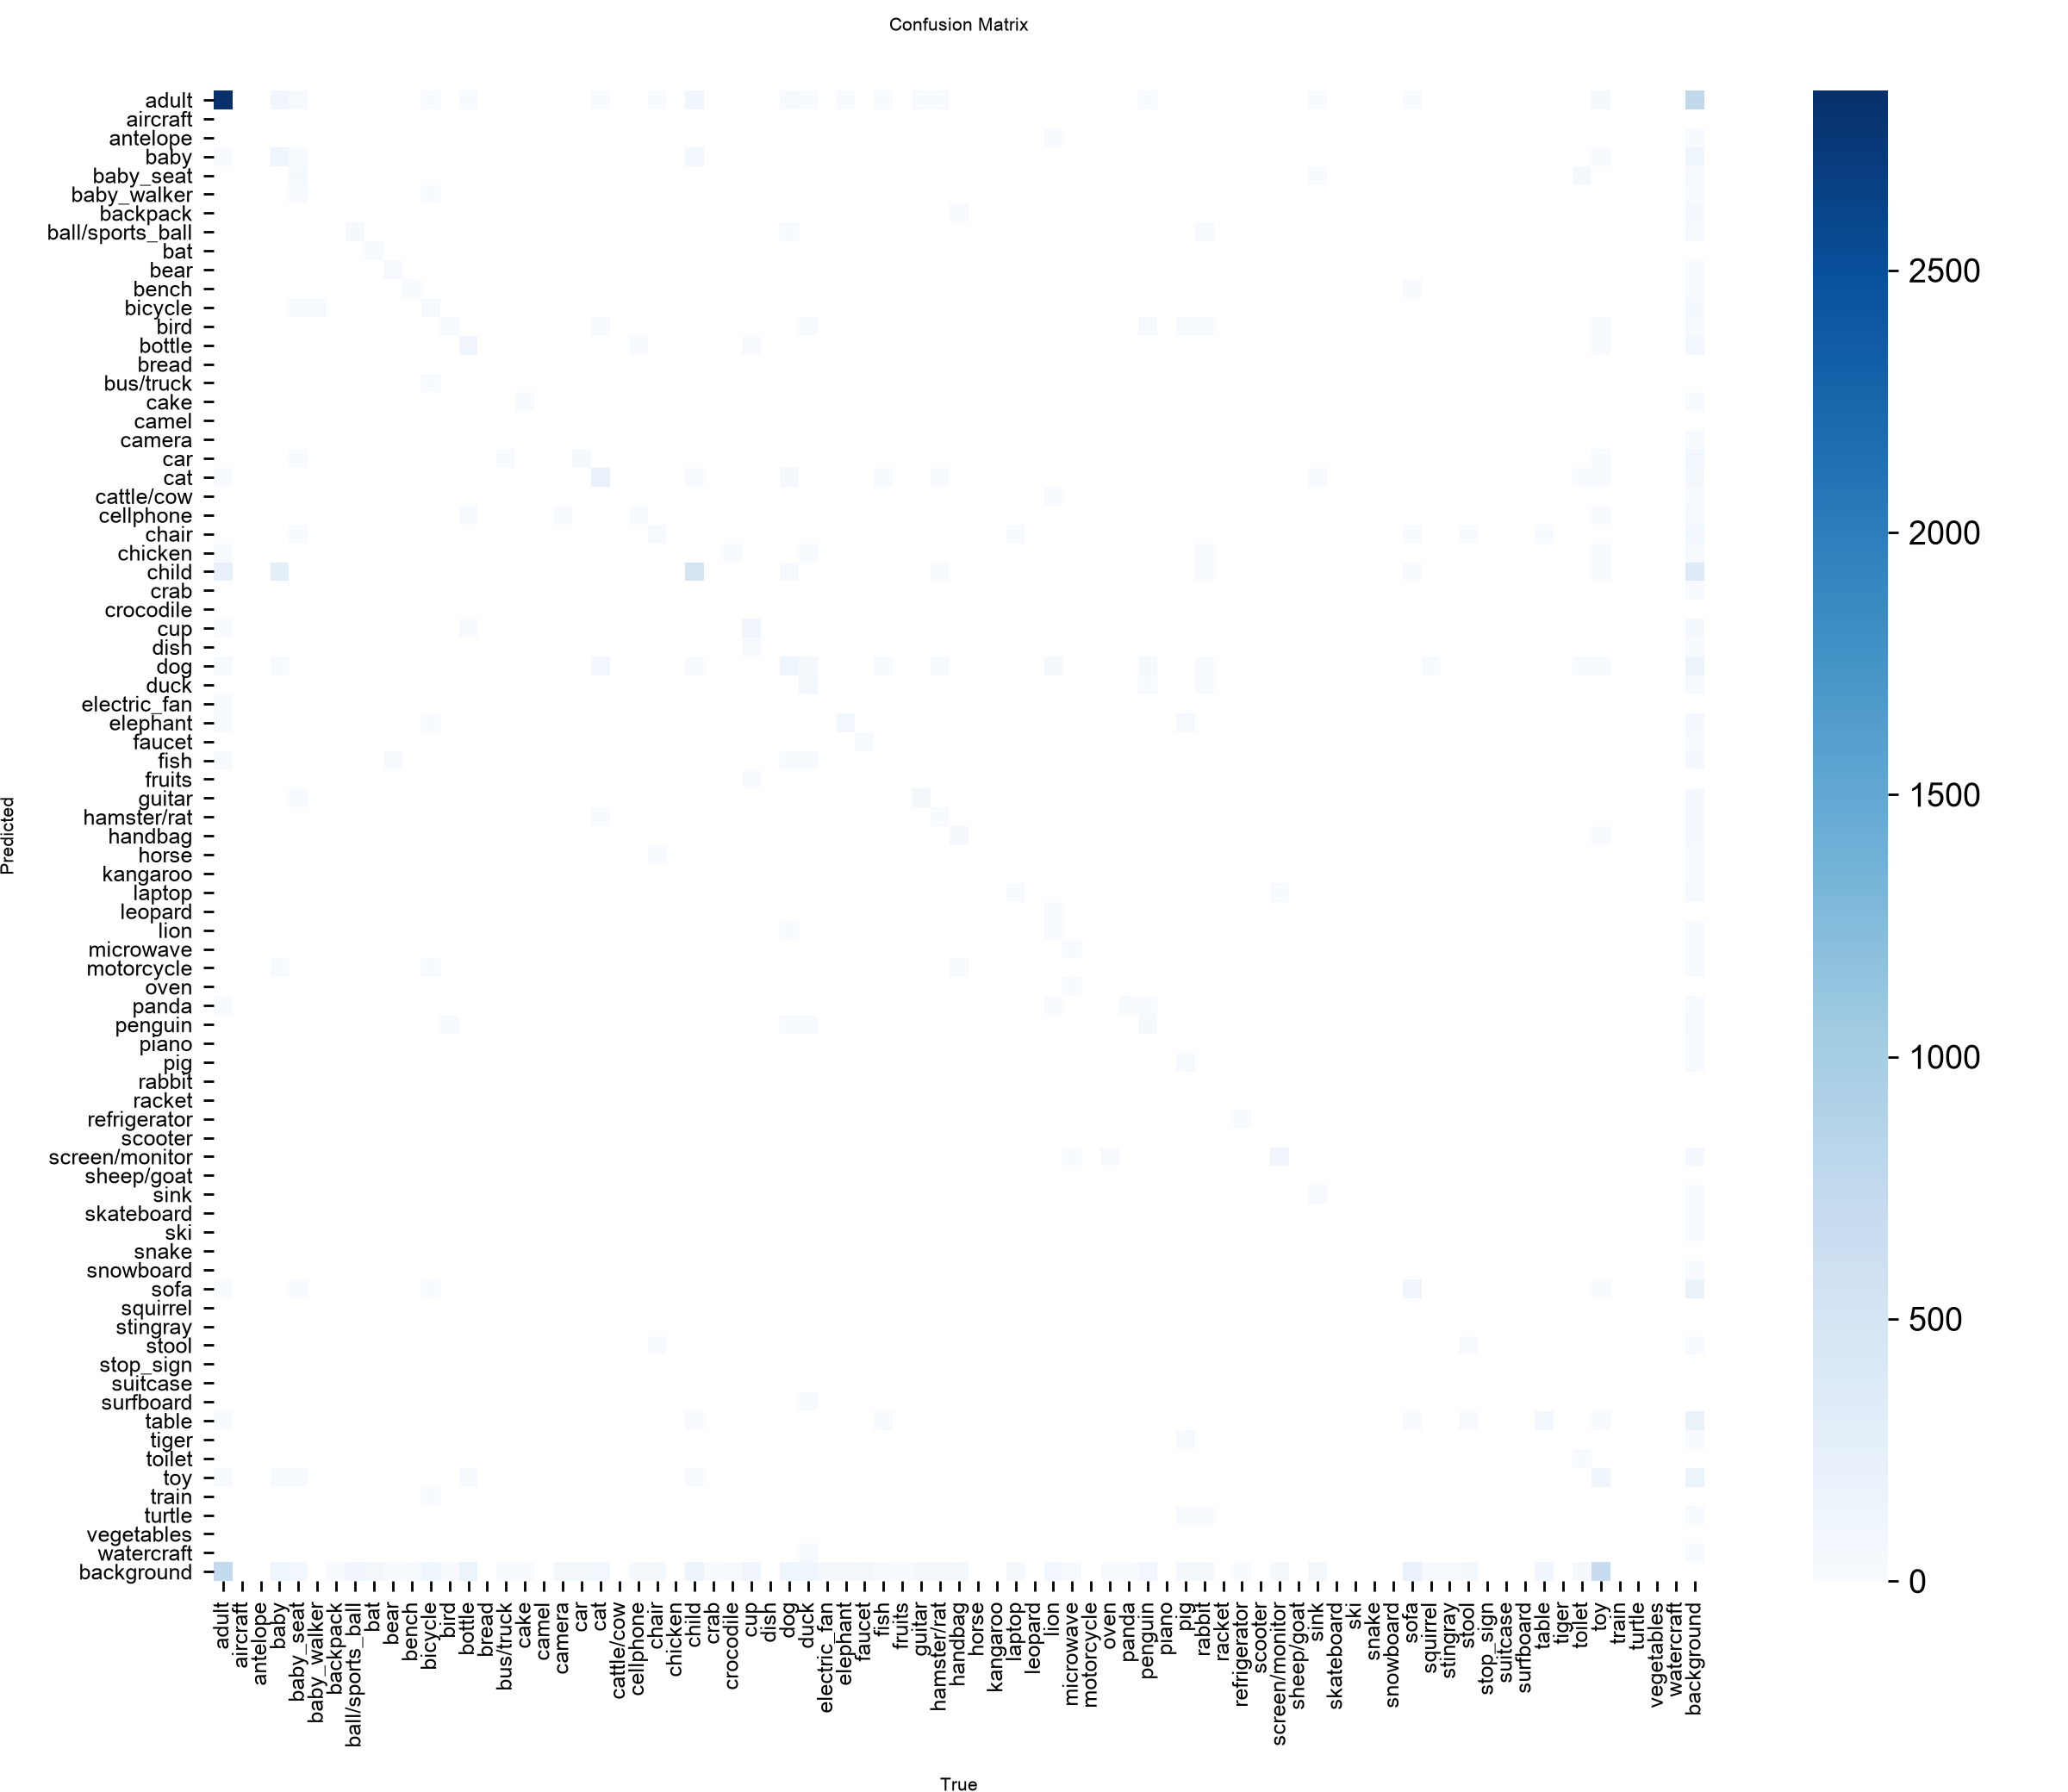
\includegraphics[width=\textwidth]{images/finetune_confusion_crop.png}\\[-2pt]
      {\scriptsize\color{mute} Confusion matrix after fine-tuning.}
  \end{columns}
\end{frame}

% ======================= 10  ERROR ANALYSIS =======================
\begin{frame}{Strong on adults, thin on most other classes}
  \centering
  \begin{columns}[T]
    \column{0.42\textwidth}
      \centering
      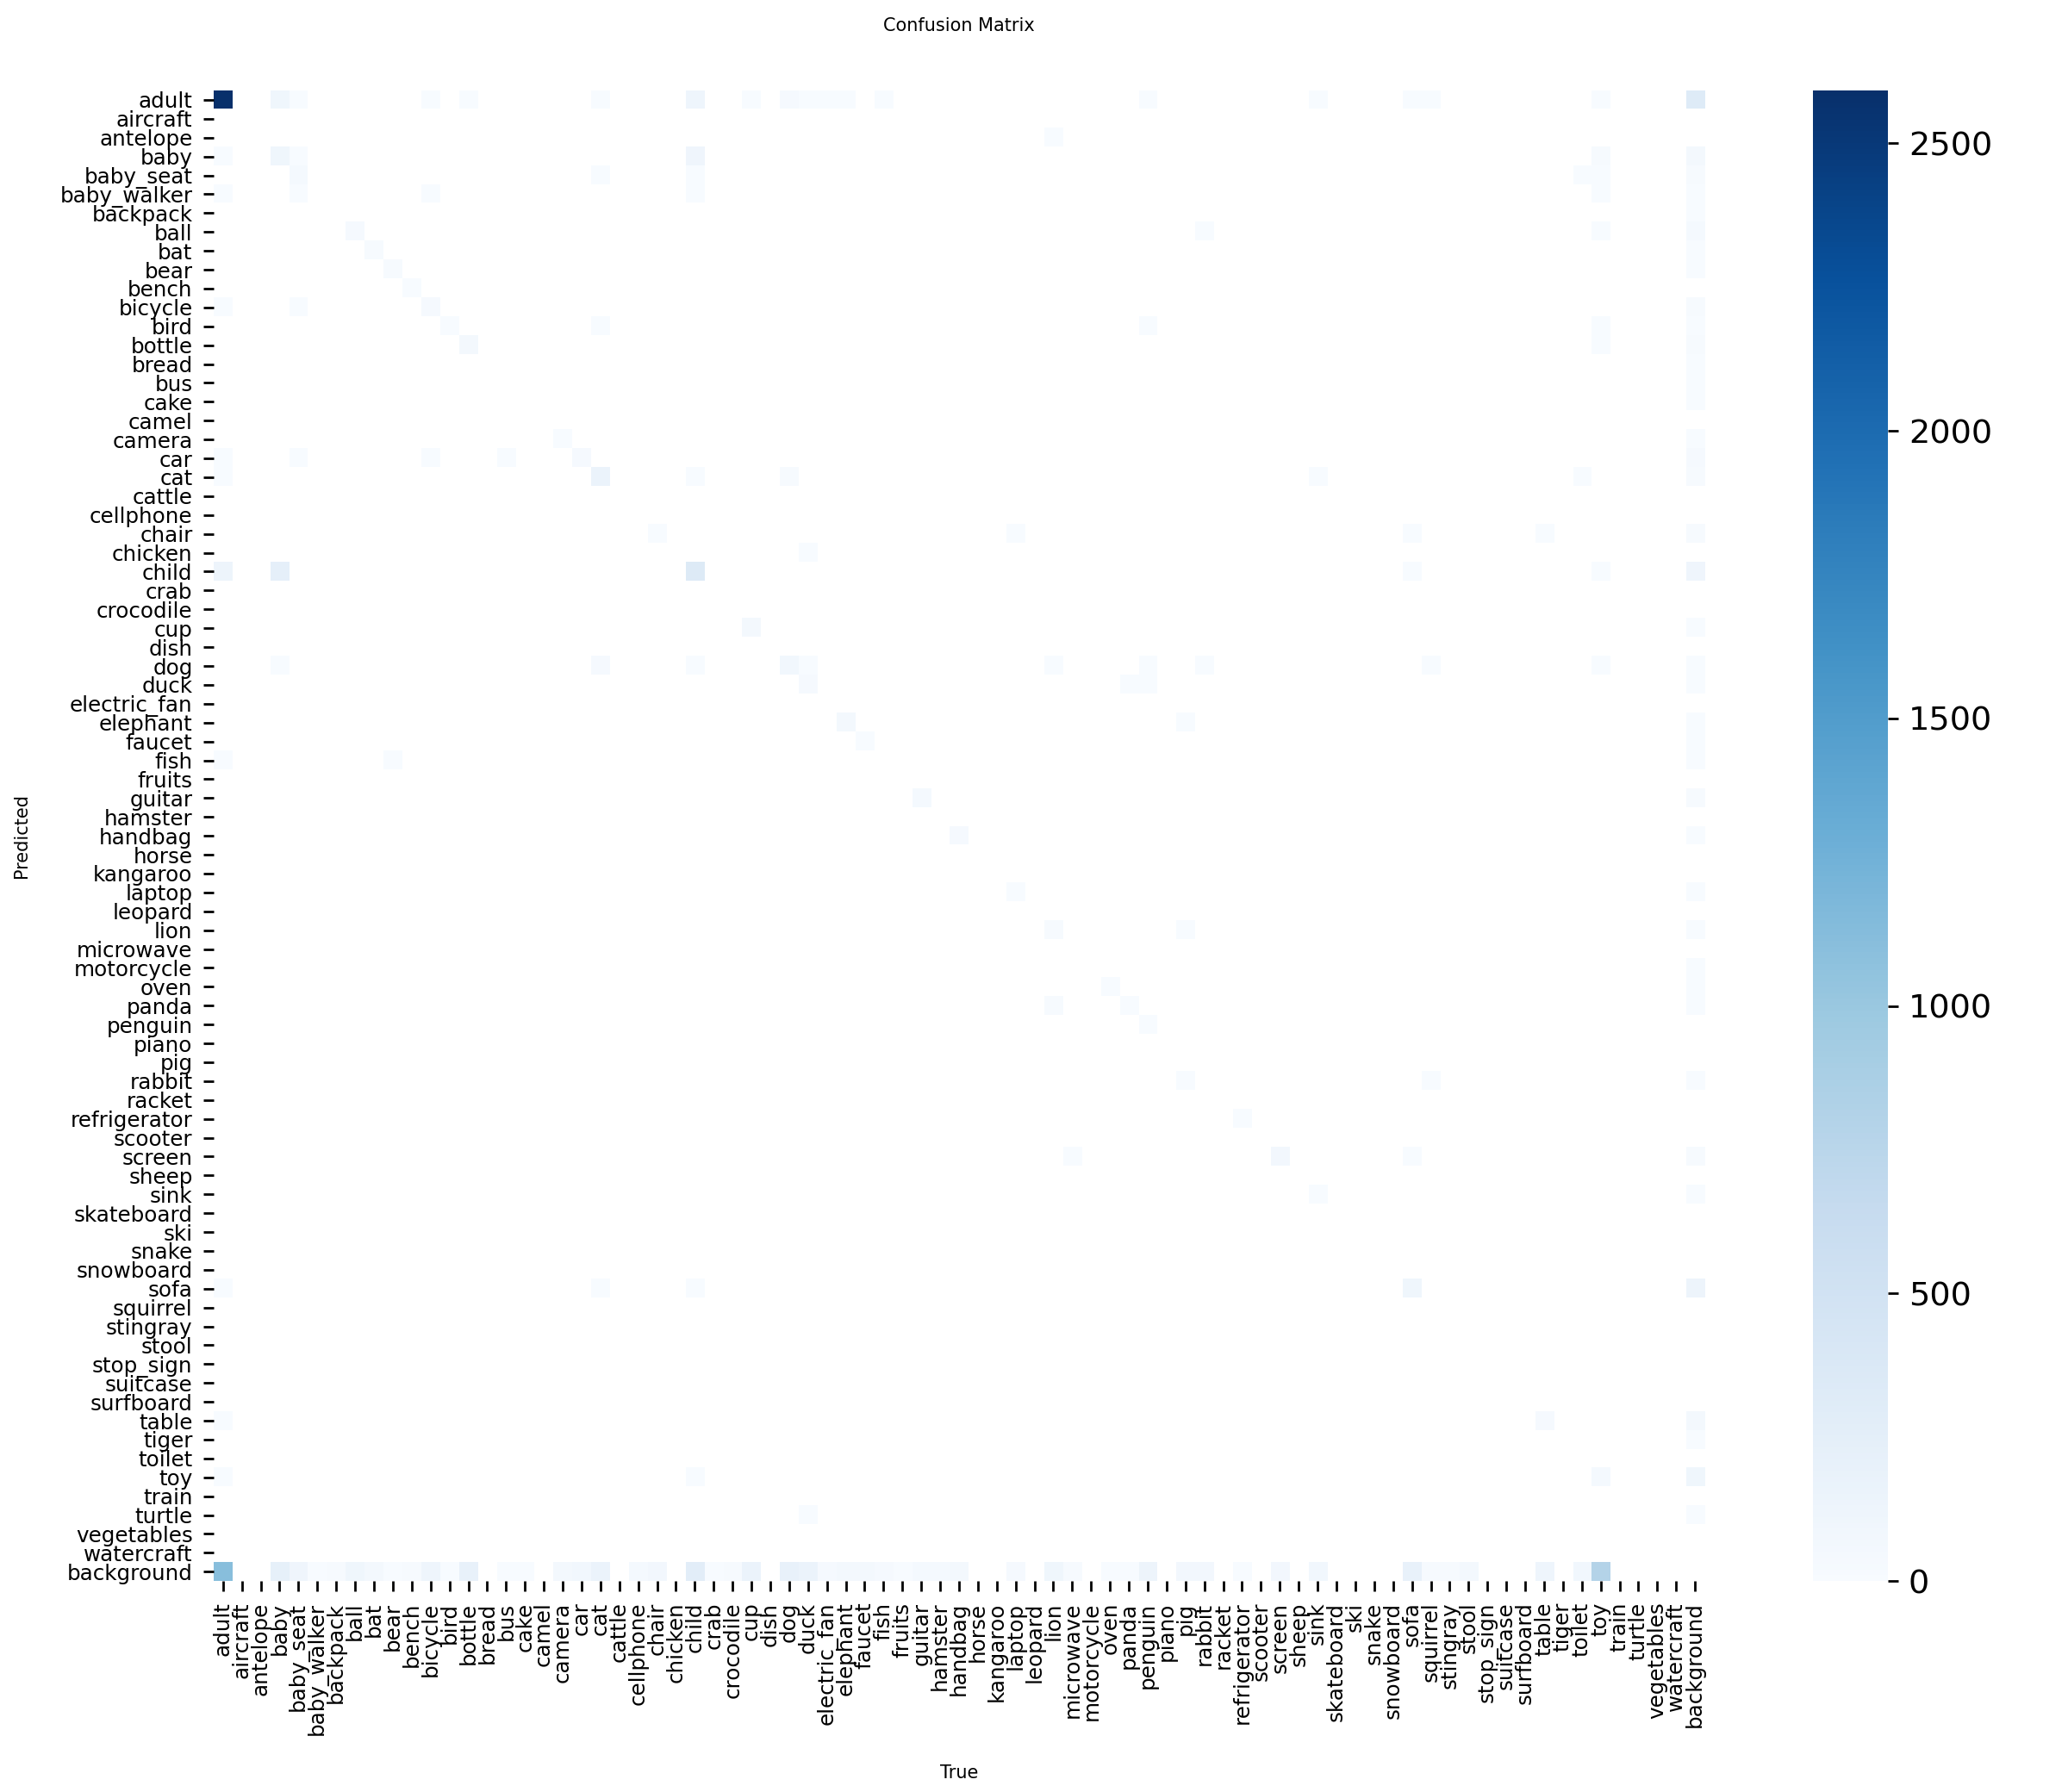
\includegraphics[width=\textwidth]{images/confusion_matrix_crop.png}\\[-2pt]
      {\scriptsize\color{mute} Confusion matrix: a dark adult cell, faint scatter elsewhere.}
    \column{0.54\textwidth}
      \centering
      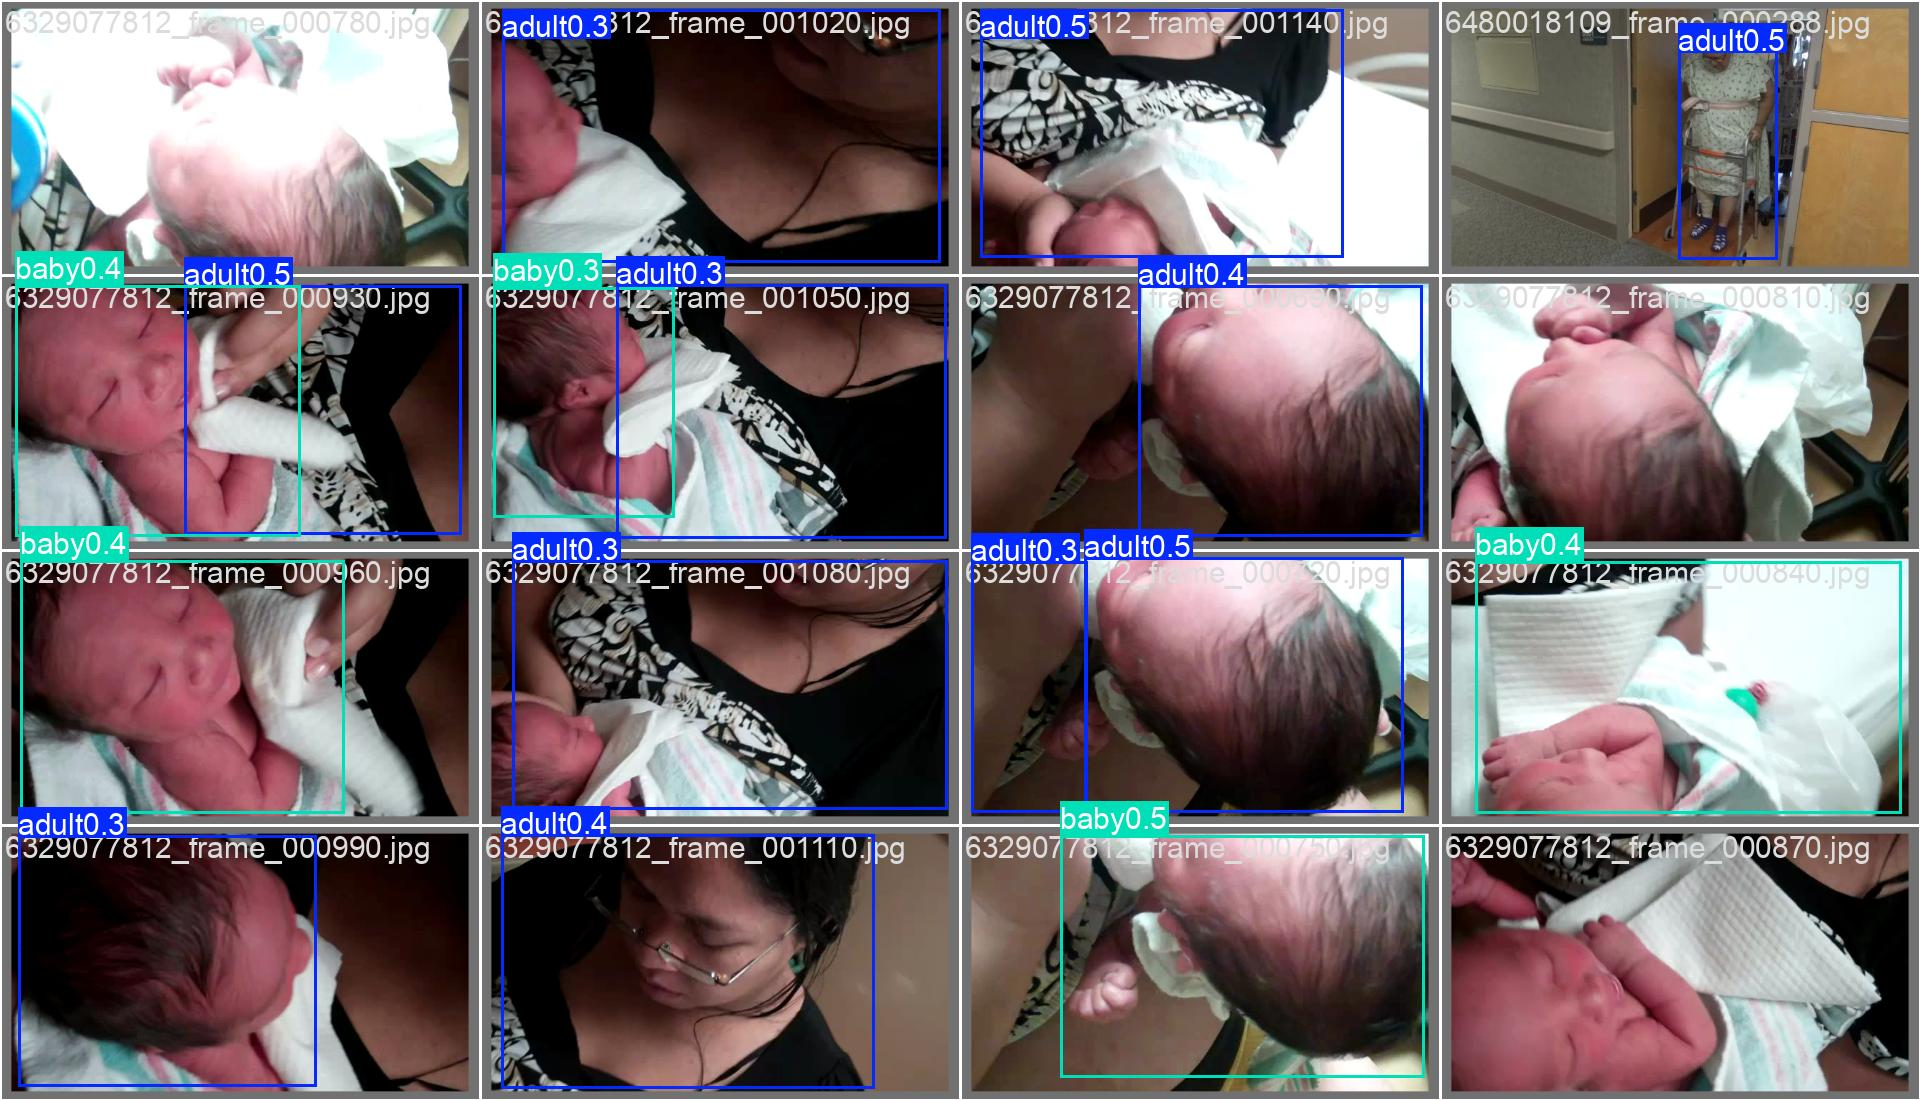
\includegraphics[width=\textwidth]{images/val_batch0_pred.jpg}\\[-2pt]
      {\scriptsize\color{mute} Validation predictions: adult and baby found, confidence 0.3--0.5.}
  \end{columns}
\end{frame}

% ======================= 10b  TRAINING GRAPHS =======================
\begin{frame}{Training graphs from the run}
  \centering
  \begin{columns}[T]
    \column{0.60\textwidth}
      \centering
      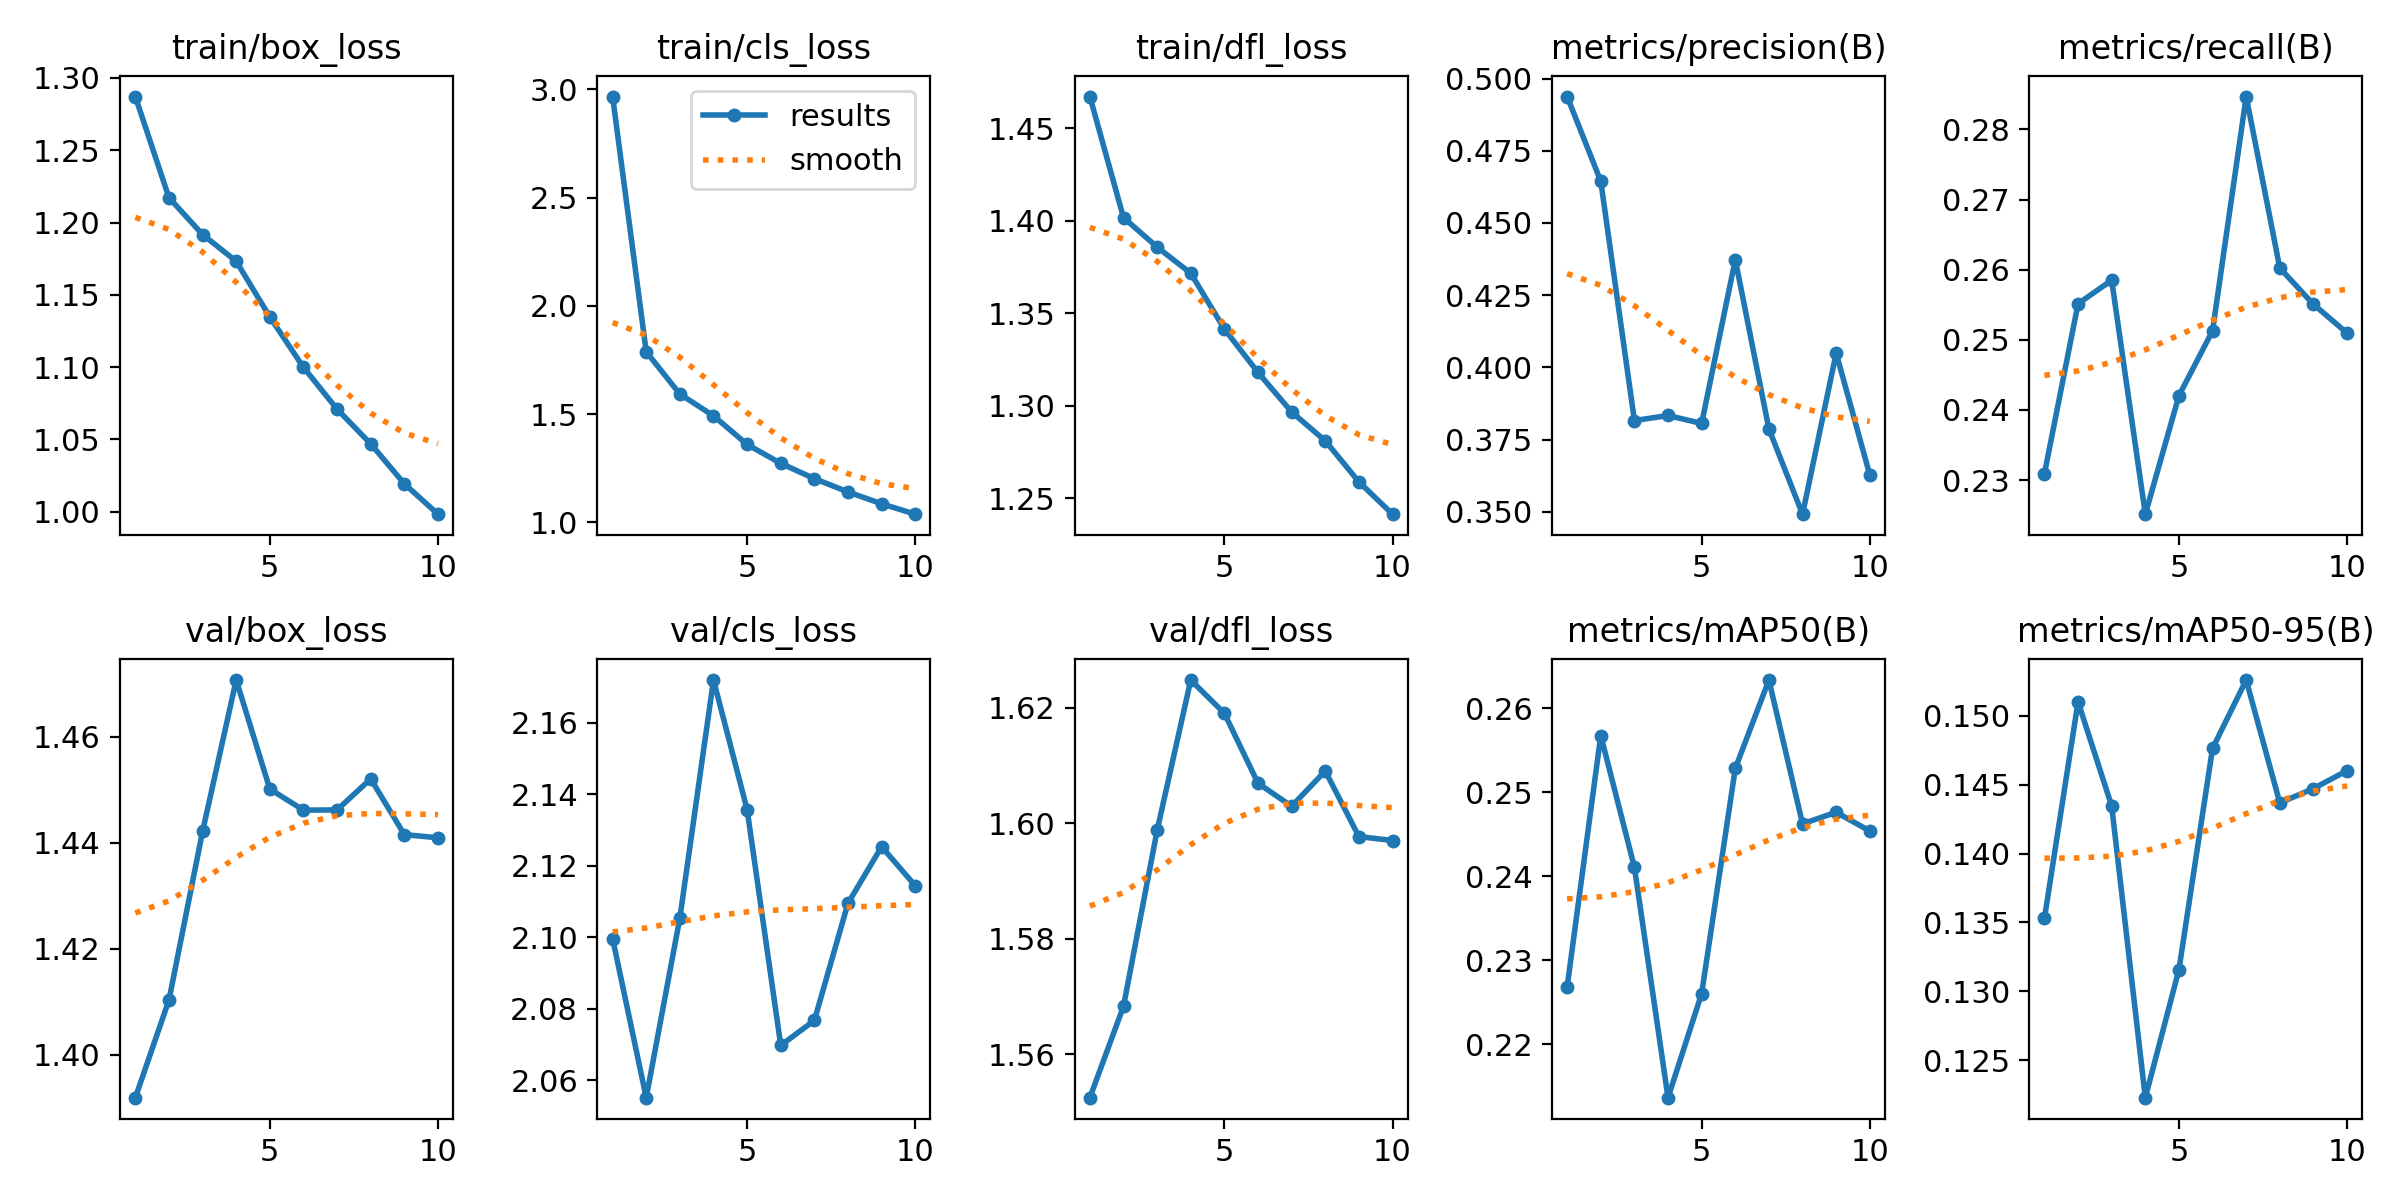
\includegraphics[width=\textwidth]{images/results.png}\\[-2pt]
      {\scriptsize\color{mute} Losses, precision, recall and mAP over the 10 epochs.}
    \column{0.36\textwidth}
      \centering
      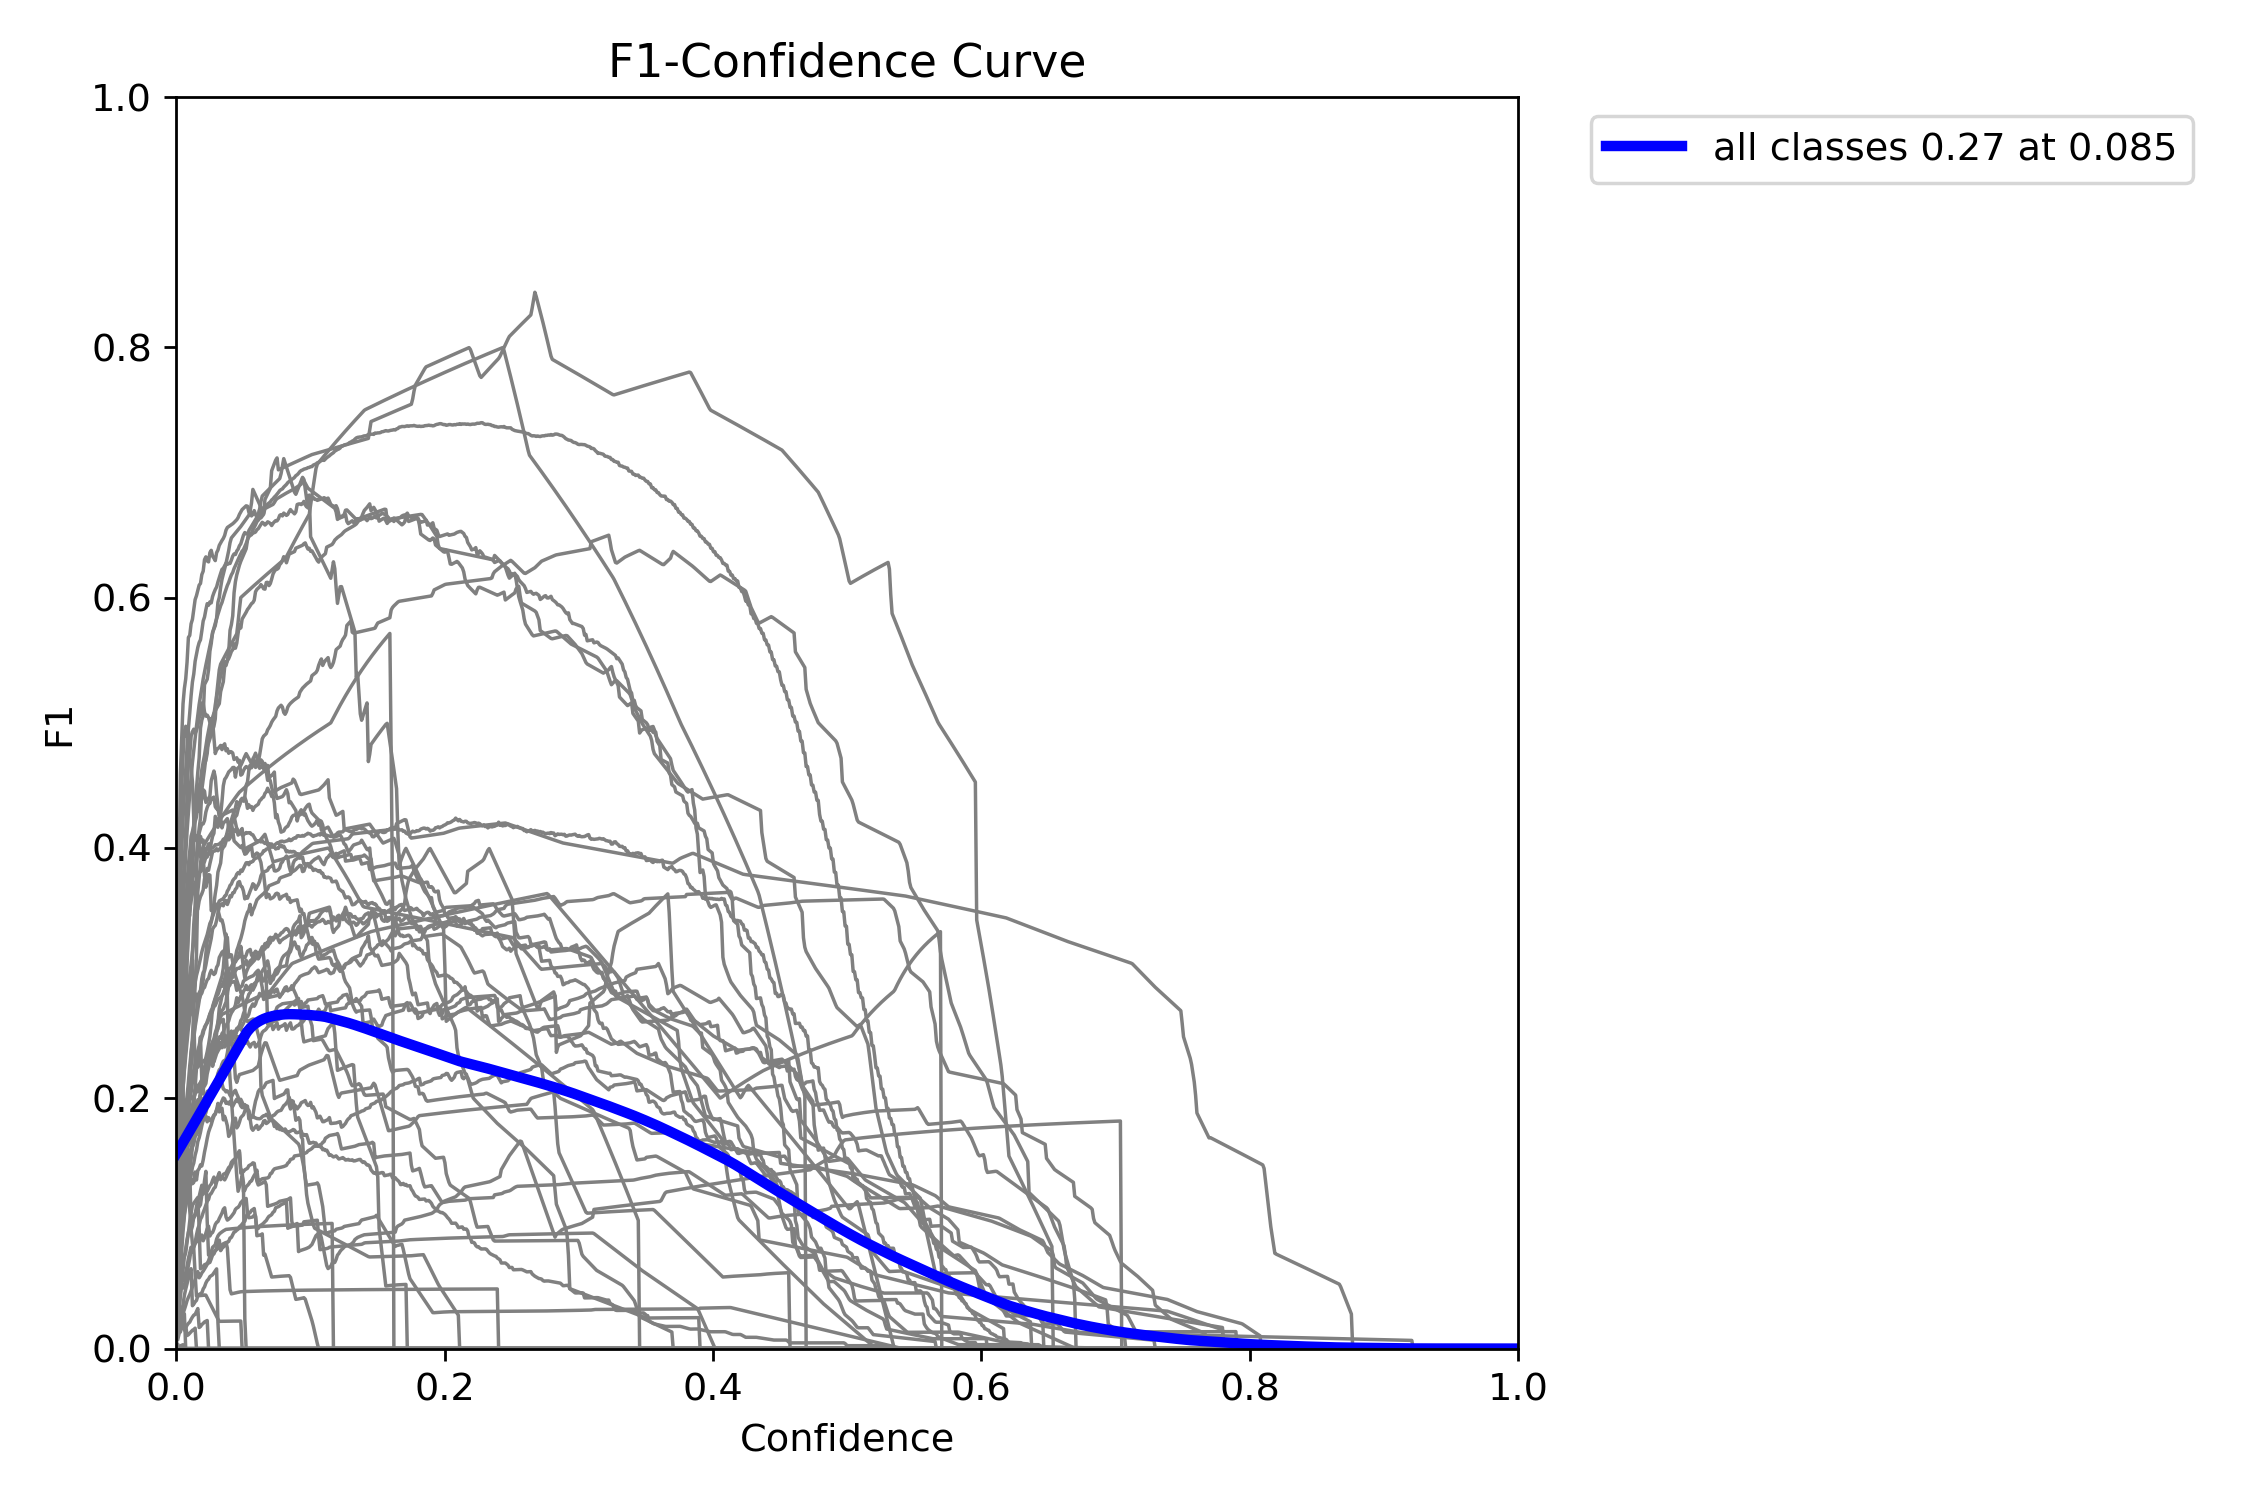
\includegraphics[width=\textwidth]{images/BoxF1_curve.png}\\[-2pt]
      {\scriptsize\color{mute} F1 versus confidence threshold.}
  \end{columns}
\end{frame}

% ======================= 11  TEMPORAL GRAPH =======================
\begin{frame}{Tracks turn per-frame boxes into a temporal graph}
  \centering
  \begin{center}
  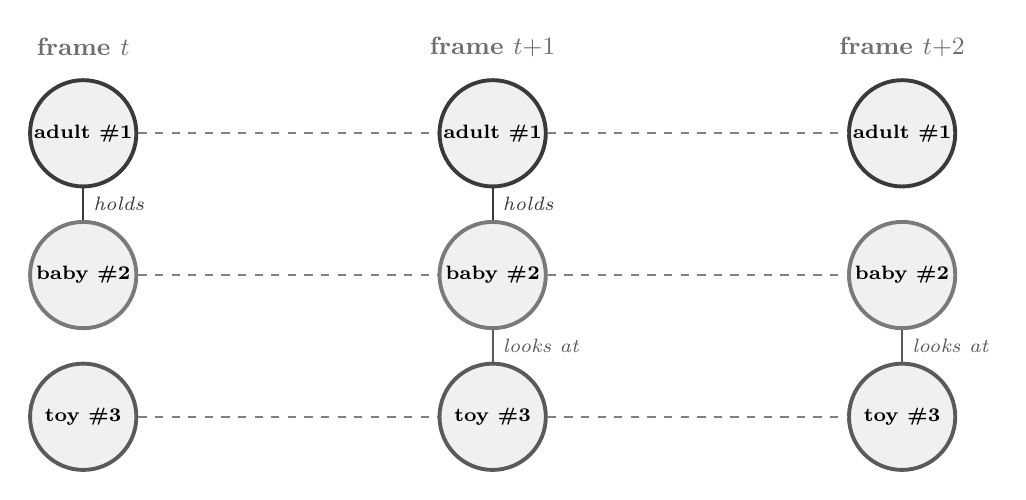
\begin{tikzpicture}[
      n/.style={circle,draw,line width=1.4pt,fill=paper,minimum size=1.35cm,font=\scriptsize\bfseries,inner sep=0pt}]
    \foreach \x/\k/\lab in {0/0/{frame $t$},5.2/1/{frame $t{+}1$},10.4/2/{frame $t{+}2$}}{
      \node[font=\small\bfseries,text=mute] at (\x,2.9) {\lab};
      \node[n,draw=amber] (a\k) at (\x,1.8) {adult \#1};
      \node[n,draw=teal]  (b\k) at (\x,0.0) {baby \#2};
      \node[n,draw=coral] (c\k) at (\x,-1.8) {toy \#3};}
    \draw[amber,thick] (a0)--(b0) node[midway,right,font=\scriptsize\itshape]{holds};
    \draw[amber,thick] (a1)--(b1) node[midway,right,font=\scriptsize\itshape]{holds};
    \draw[coral,thick] (b1)--(c1) node[midway,right,font=\scriptsize\itshape]{looks at};
    \draw[coral,thick] (b2)--(c2) node[midway,right,font=\scriptsize\itshape]{looks at};
    \foreach \id in {a,b,c}{
      \draw[dashed,thick,gray] (\id0)--(\id1);
      \draw[dashed,thick,gray] (\id1)--(\id2);}
  \end{tikzpicture}
  \end{center}
  {\small Solid edges: relations inside a frame. Dashed edges: the same object linked through time.}
\end{frame}

% ======================= 12  RELATION DATA =======================
\begin{frame}{Relation samples come from tracks and features}
  \centering
  \begin{center}
  \resizebox{\textwidth}{!}{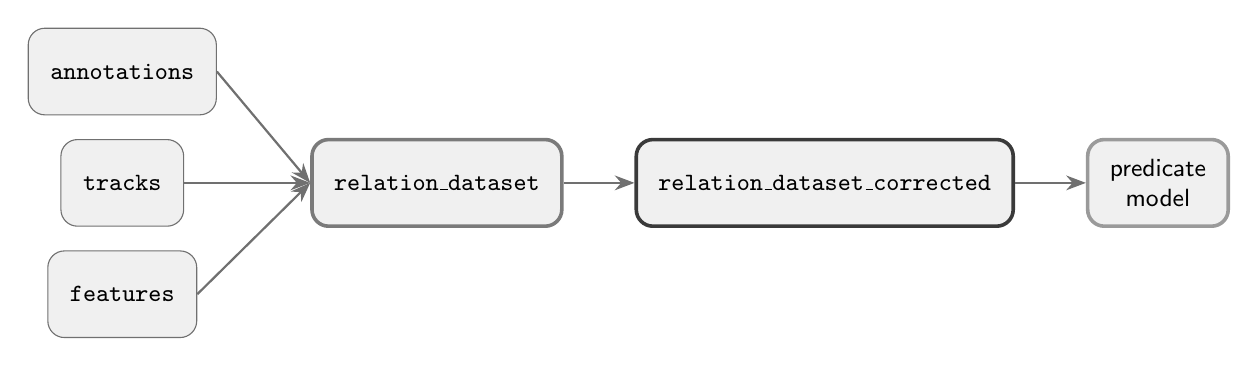
\begin{tikzpicture}[node distance=0.9cm,
      b/.style={rounded corners=6pt,draw=navy!60,fill=paper,minimum height=1.1cm,align=center,font=\small\ttfamily,inner xsep=8pt},
      ar/.style={-{Stealth[length=2.5mm]},thick,navy!60}]
    \node[b] (an) {annotations};
    \node[b,below=0.3cm of an] (tr) {tracks};
    \node[b,below=0.3cm of tr] (fe) {features};
    \node[b,draw=teal,line width=1.3pt,right=1.6cm of tr] (r1) {relation\_dataset};
    \node[b,draw=amber,line width=1.3pt,right=0.9cm of r1] (r2) {relation\_dataset\_corrected};
    \node[b,draw=peri,line width=1.3pt,right=0.9cm of r2,font=\small\sffamily] (pm) {predicate\\model};
    \draw[ar] (an.east) -- (r1.west); \draw[ar] (tr.east) -- (r1.west); \draw[ar] (fe.east) -- (r1.west);
    \draw[ar] (r1)--(r2); \draw[ar] (r2)--(pm);
  \end{tikzpicture}}
  \end{center}
  {\small Two exports exist: the first relation set and a corrected version. The corrected one is the cleaner input for relation learning.}
\end{frame}

% ======================= COMBINING OLD AND NEW =======================
\begin{frame}{Combining old and new training: 28 to 78 classes}
  \centering
  \begin{center}
  \resizebox{\textwidth}{!}{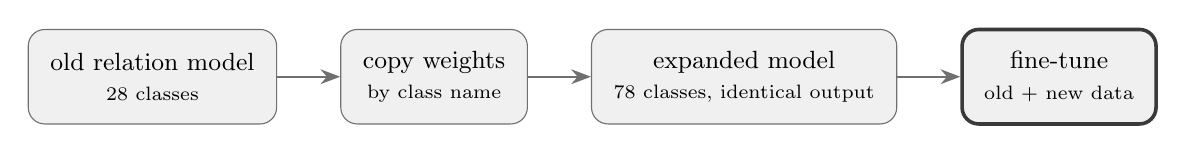
\begin{tikzpicture}[node distance=0.8cm,
      b/.style={rounded corners=6pt,draw=navy!60,fill=paper,minimum height=1.2cm,align=center,font=\small,inner xsep=8pt},
      ar/.style={-{Stealth[length=2.5mm]},thick,navy!60}]
    \node[b] (old) {old relation model\\\scriptsize 28 classes};
    \node[b,right=of old] (map) {copy weights\\\scriptsize by class name};
    \node[b,right=of map] (new) {expanded model\\\scriptsize 78 classes, identical output};
    \node[b,right=of new,draw=amber,line width=1.3pt] (ft) {fine-tune\\\scriptsize old + new data};
    \draw[ar] (old)--(map); \draw[ar] (map)--(new); \draw[ar] (new)--(ft);
  \end{tikzpicture}}
  \end{center}
  \small
  \begin{tabular}{lrrr}
    \toprule
    & Old data & New data & Combined\\
    \midrule
    Relation training pairs & 7,536 & 145,031 & 152,567\\
    Temporal training sequences & 1,890 & 38,388 & 40,278\\
    \bottomrule
  \end{tabular}\\[6pt]
  {\footnotesize The expanded model gave exactly the same answers as the old one on the old validation set (accuracy 0.429, loss 1.758), so no knowledge was lost. 38 new videos (every 10th) were held out of training to test on unseen data.}
\end{frame}

% ======================= RELATION + TEMPORAL RESULTS =======================
\begin{frame}[t]{Relation and temporal models: before $\rightarrow$ after fine-tuning}
  \centering\vspace{0.3cm}\scriptsize
  \begin{tabular}{llccc}
    \toprule
    Model & Test set & Accuracy & Macro-F1 & Loss\\
    \midrule
Relation & old val & 0.429 $\rightarrow$ 0.529 & 0.068 $\rightarrow$ 0.077 & 1.758 $\rightarrow$ 1.490\\
    Relation & new videos & 0.303 $\rightarrow$ 0.407 & 0.098 $\rightarrow$ 0.124 & 2.264 $\rightarrow$ 1.781\\
    Temporal LSTM & old val & 0.645 $\rightarrow$ 0.586 & 0.072 $\rightarrow$ 0.099 & 1.317 $\rightarrow$ 1.375\\
    Temporal LSTM & new videos & 0.278 $\rightarrow$ 0.372 & 0.026 $\rightarrow$ 0.074 & 2.100 $\rightarrow$ 1.891\\
    Temporal GRU & old val & 0.576 $\rightarrow$ 0.628 & 0.075 $\rightarrow$ 0.113 & 1.510 $\rightarrow$ 1.372\\
    Temporal GRU & new videos & 0.281 $\rightarrow$ 0.390 & 0.032 $\rightarrow$ 0.063 & 2.284 $\rightarrow$ 1.809\\
    \bottomrule
  \end{tabular}\\[5pt]
  \begin{minipage}{0.92\textwidth}\scriptsize
  \begin{itemize}\setlength\itemsep{1pt}
    \item Every model improves on the unseen new videos; the old models had never seen most of the 78 classes.
    \item The LSTM is slightly worse on the old validation set (accuracy 0.645 $\rightarrow$ 0.586); the GRU improves on both.
    \item Scores are still low: macro-F1 is at most 0.13, because background pairs dominate the data.
    \item Validation loss is best after 1 to 3 epochs, then rises (over-fitting), so early stopping chose the checkpoints.
  \end{itemize}
  \end{minipage}
\end{frame}

% ======================= WHY TWO PREDICATES DOMINATED =======================
\begin{frame}[t]{Why two predicates dominated the graphs}
  \centering\vspace{0.2cm}
  \begin{columns}[T]
    \column{0.50\textwidth}
      \centering
      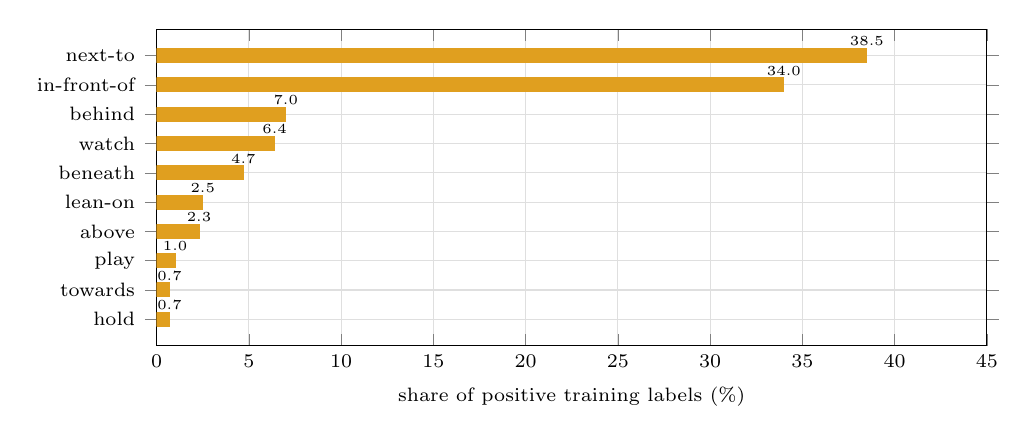
\begin{tikzpicture}
        \begin{axis}[xbar,width=\textwidth,height=5.6cm,xmin=0,xmax=45,bar width=5pt,
          symbolic y coords={hold,towards,play,above,lean-on,beneath,watch,behind,in-front-of,next-to},ytick=data,
          y tick label style={font=\scriptsize},x tick label style={font=\scriptsize},xlabel={\scriptsize share of positive training labels (\%)},
          nodes near coords,nodes near coords style={font=\tiny},point meta=explicit symbolic,grid=major,grid style={gray!25}]
          \addplot[fill=cAmber,draw=cAmber] coordinates {(0.7,hold) [0.7] (0.7,towards) [0.7] (1.0,play) [1.0] (2.3,above) [2.3] (2.5,lean-on) [2.5] (4.7,beneath) [4.7] (6.4,watch) [6.4] (7.0,behind) [7.0] (34.0,in-front-of) [34.0] (38.5,next-to) [38.5]};
        \end{axis}
      \end{tikzpicture}
    \column{0.47\textwidth}
      \footnotesize
      \begin{itemize}\setlength\itemsep{3pt}
        \item \textbf{Data:} next\_to and in\_front\_of are \textbf{72\%} of all positive labels; the rarest predicates have fewer than 30 samples.
        \item \textbf{Loss:} v1 used an unweighted loss, so guessing the common classes pays off.
        \item \textbf{Checkpoints:} v1 was chosen by validation loss, but macro-F1 on new videos was still rising (0.124 $\rightarrow$ 0.156 by epoch 5).
        \item \textbf{Result:} v1 predicted only 11 of 32 predicates (the GRU only 4).
      \end{itemize}
  \end{columns}
\end{frame}

% ======================= THE FIX: V1 VS V2 =======================
\begin{frame}[t]{The fix: class-balanced loss, checkpoints chosen by macro-F1}
  \centering\vspace{0.2cm}\scriptsize\setlength{\tabcolsep}{3.5pt}
  \begin{tabular}{llcccc}
    \toprule
    Model & Test set & Macro-F1 & Accuracy & Predicates used & Top-2 share\\
    \midrule
    Relation & new videos & 0.124 $\rightarrow$ 0.189 & 0.407 $\rightarrow$ 0.406 & 11 $\rightarrow$ 23 & 74\% $\rightarrow$ 58\%\\
    Relation & old val & 0.084 $\rightarrow$ 0.064 & 0.529 $\rightarrow$ 0.314 & 8 $\rightarrow$ 14 & 73\% $\rightarrow$ 53\%\\
    Temporal LSTM & new videos & 0.074 $\rightarrow$ 0.145 & 0.372 $\rightarrow$ 0.339 & 8 $\rightarrow$ 17 & 95\% $\rightarrow$ 54\%\\
    Temporal LSTM & old val & 0.099 $\rightarrow$ 0.059 & 0.586 $\rightarrow$ 0.322 & 4 $\rightarrow$ 10 & 92\% $\rightarrow$ 47\%\\
    Temporal GRU & new videos & 0.063 $\rightarrow$ 0.172 & 0.390 $\rightarrow$ 0.333 & 4 $\rightarrow$ 22 & 99\% $\rightarrow$ 45\%\\
    Temporal GRU & old val & 0.113 $\rightarrow$ 0.130 & 0.628 $\rightarrow$ 0.396 & 3 $\rightarrow$ 13 & 100\% $\rightarrow$ 49\%\\
    \bottomrule
  \end{tabular}\\[6pt]
  \begin{minipage}{0.93\textwidth}\scriptsize
  \begin{itemize}\setlength\itemsep{1pt}
    \item v2 = v1 retrained with loss weights $\propto 1/\sqrt{\mathrm{frequency}}$ (capped at 12$\times$), checkpoint chosen by macro-F1. ``Top-2 share'' = share of non-background predictions that are next\_to or in\_front\_of.
    \item On new videos every model gains macro-F1 and uses far more predicates; the GRU's top-2 share falls from 99\% to 45\%.
    \item Cost: accuracy drops (it rewarded guessing common classes). On the small old validation set the result is mixed: relation worse, LSTM worse, GRU better.
  \end{itemize}
  \end{minipage}
\end{frame}

% ======================= V2 GRAPHS =======================
\begin{frame}[t]{Dynamic scene graphs after the fix (1/2)}
  \centering\vspace{0.1cm}
  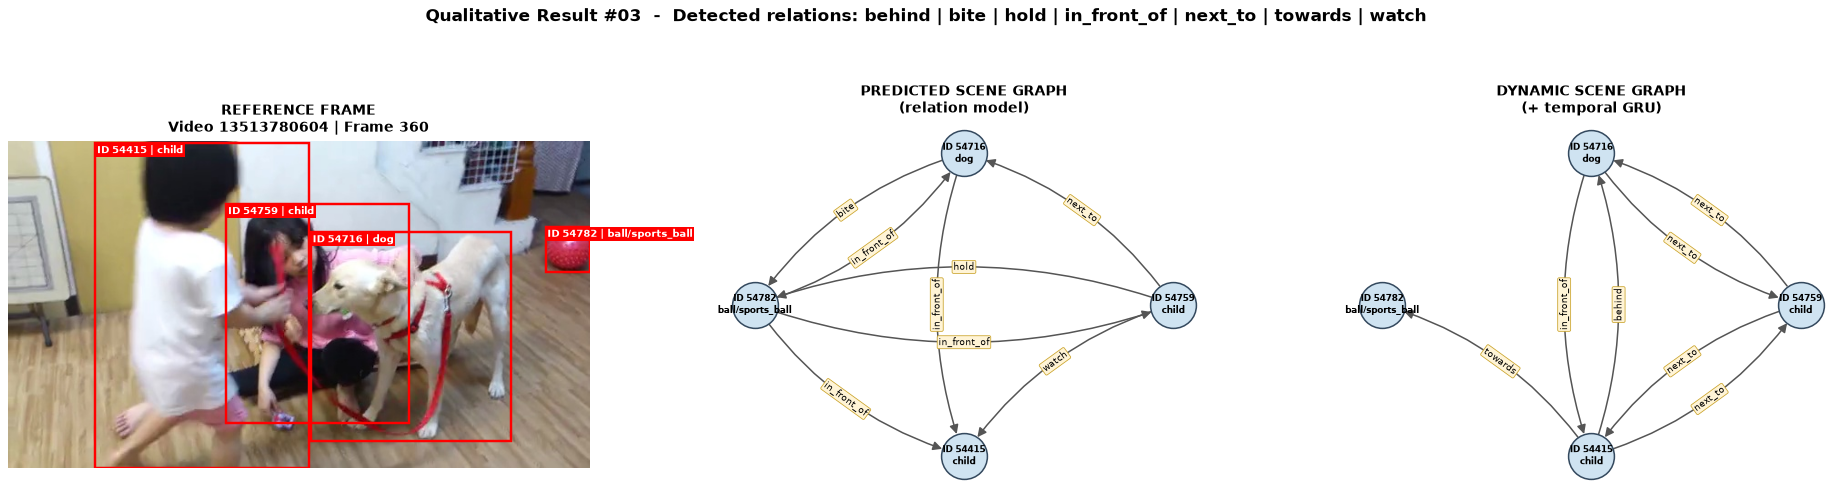
\includegraphics[width=0.80\textwidth]{images/v2_graph_1_trim.png}\\[1pt]
  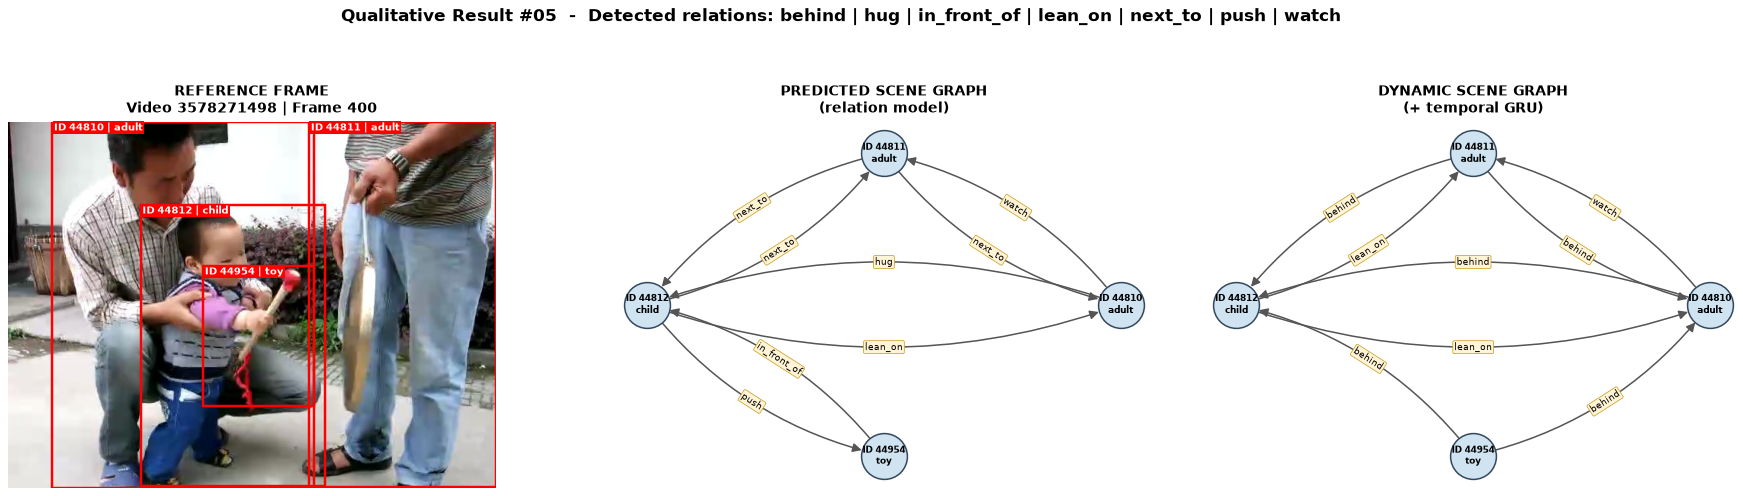
\includegraphics[width=0.80\textwidth]{images/v2_graph_2_trim.png}\\[-1pt]
  {\scriptsize\color{mute} Held-out new videos. Examples were picked for predicate variety, not at random.}
\end{frame}

\begin{frame}[t]{Dynamic scene graphs after the fix (2/2)}
  \centering\vspace{0.1cm}
  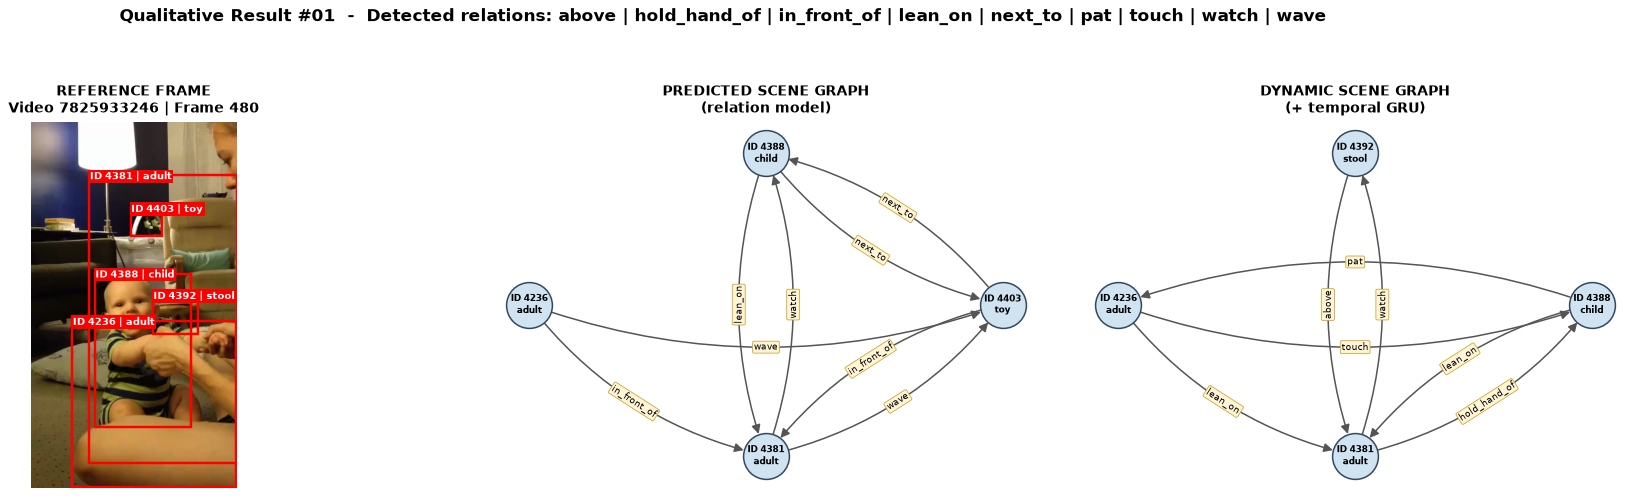
\includegraphics[width=0.70\textwidth]{images/v2_graph_3_trim.png}\\[1pt]
  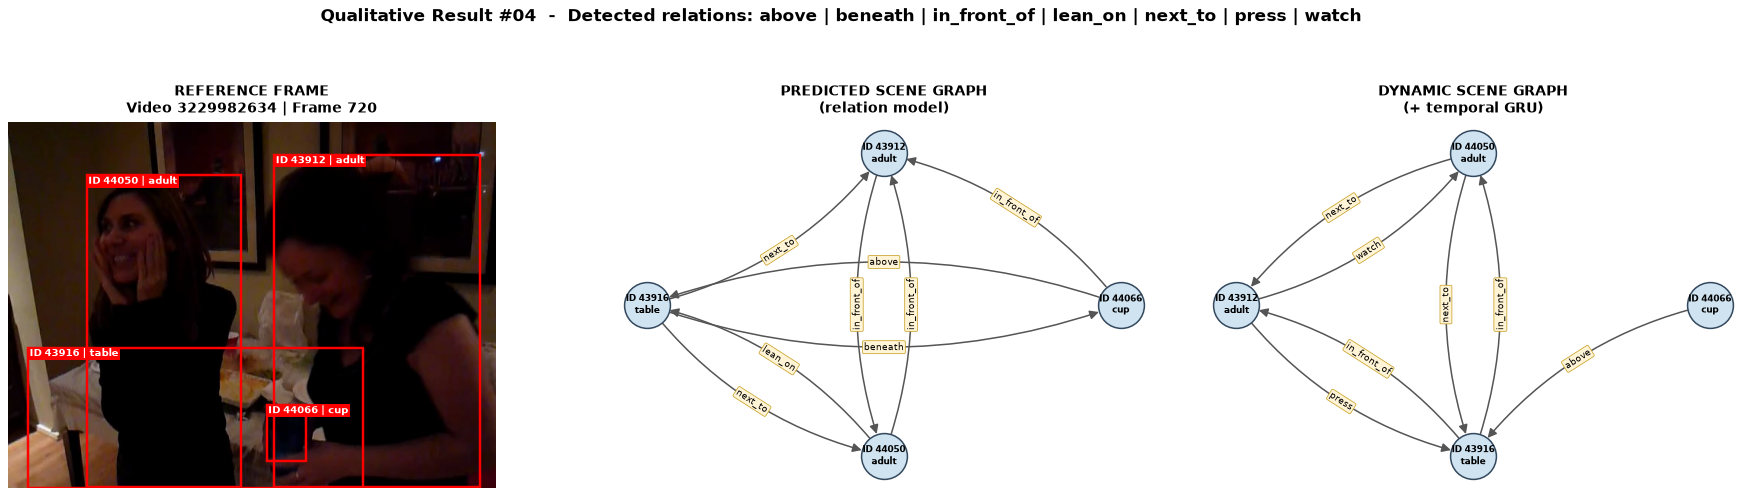
\includegraphics[width=0.74\textwidth]{images/v2_graph_4_trim.png}\\[-1pt]
  {\scriptsize\color{mute} Some relations are plausible (watch, hold, towards), others are wrong: scores remain low.}
\end{frame}

% ======================= QUALITATIVE RESULTS =======================
\begin{frame}[t]{Qualitative results: frames and predicted graphs}
  \centering\vspace{0.25cm}
  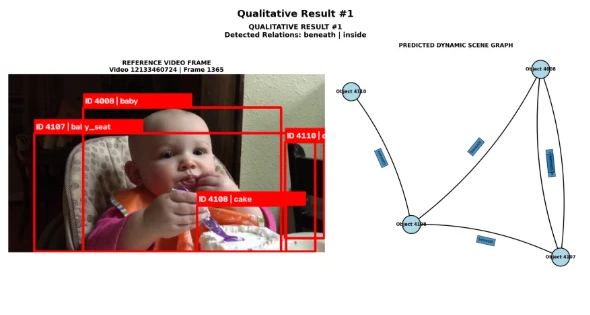
\includegraphics[width=0.43\textwidth]{images/qual_q1.png}\hfill
  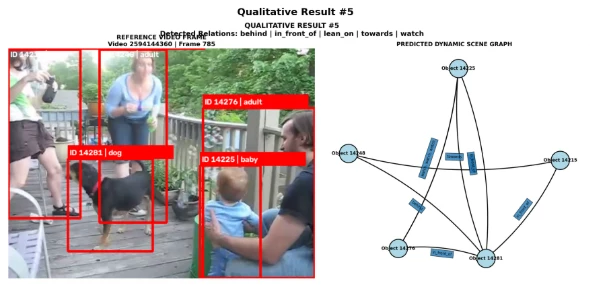
\includegraphics[width=0.43\textwidth]{images/qual_q5.png}\\[0pt]
  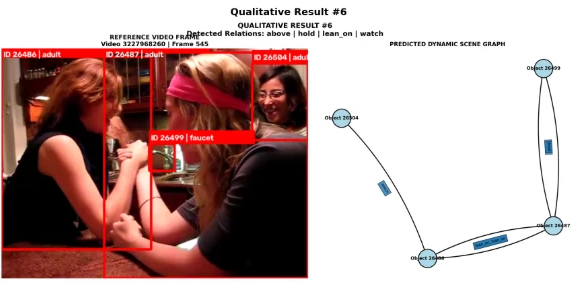
\includegraphics[width=0.43\textwidth]{images/qual_q6.png}\hfill
  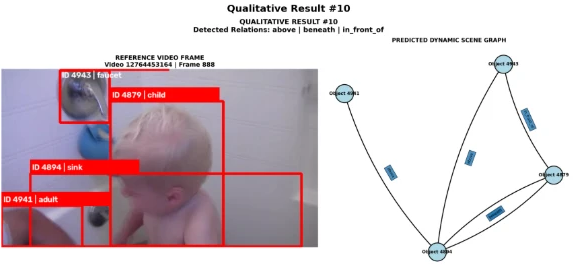
\includegraphics[width=0.43\textwidth]{images/qual_q10.png}\\[-2pt]
  {\scriptsize\color{mute} Left: tracked, labelled objects. Right: predicted scene graph with relation labels.}
\end{frame}

% ======================= 13  LESSONS =======================
\begin{frame}{What slowed us down and what we learned}
  \centering
  \vspace{0.3cm}\large
  \begin{columns}[T]
    \column{0.48\textwidth}
      \centering
      \begin{block}{1 \ Compute}
        Limited GPU access: the final fine-tune ran on a Mac, about 4 hours for 3 epochs.
      \end{block}
      \begin{block}{2 \ Class mismatch}
        The pipeline had 28 classes, the detector 78. Fixed by expanding by class name.
      \end{block}
    \column{0.48\textwidth}
      \centering
      \begin{block}{3 \ Over-fitting}
        Relation and temporal validation loss rises after 1 to 3 epochs.
      \end{block}
      \begin{block}{4 \ Low scores}
        Detector recall is 0.30 and macro-F1 is at most 0.13.
      \end{block}
  \end{columns}
\end{frame}

% ======================= 14  REVIEW 3 =======================
\begin{frame}{Review 3: VidOR training progress}
  \centering
  \begin{center}\vspace{0.2cm}
  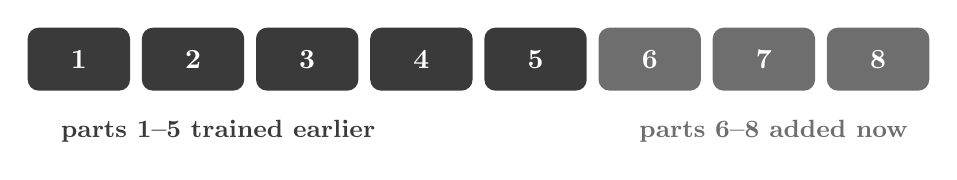
\begin{tikzpicture}
    \foreach \i in {1,...,5}{
      \node[fill=amber,rounded corners=4pt,minimum width=1.3cm,minimum height=0.8cm,text=white,font=\bfseries] at (\i*1.45,0) {\i};}
    \foreach \i in {6,...,8}{
      \node[fill=mute,rounded corners=4pt,minimum width=1.3cm,minimum height=0.8cm,text=white,font=\bfseries] at (\i*1.45,0) {\i};}
    \node[font=\small\bfseries,text=amber,anchor=north west] at (1.1,-0.65) {parts 1--5 trained earlier};
    \node[font=\small\bfseries,text=mute,anchor=north east] at (12.1,-0.65) {parts 6--8 added now};
  \end{tikzpicture}\\[12pt]
  \footnotesize
  \begin{tabular}{@{}lll@{}}
    \toprule
    \textbf{Stage} & \textbf{Before (parts 1--5)} & \textbf{After (parts 6--8 added)}\\
    \midrule
    Detector mAP50 / mAP50-95 & 0.2635 / 0.1526 & 0.2602 / 0.1548\\
    Detector recall & 0.285 & 0.303\\
    Relation, new videos (acc / macro-F1) & 0.303 / 0.098 & 0.408 / 0.124\\
    Temporal GRU, new videos (acc / macro-F1) & 0.281 / 0.032 & 0.390 / 0.063\\
    \bottomrule
  \end{tabular}
  \end{center}
  {\small\bfseries\color{amber} Honest summary: }{\small more data did not raise detector mAP50; the relation and temporal models improved on unseen new videos, but scores remain low.}
\end{frame}

% ======================= 15  NEXT =======================
\begin{frame}{Next: evaluate end to end, then improve}
  \centering
  \begin{center}
  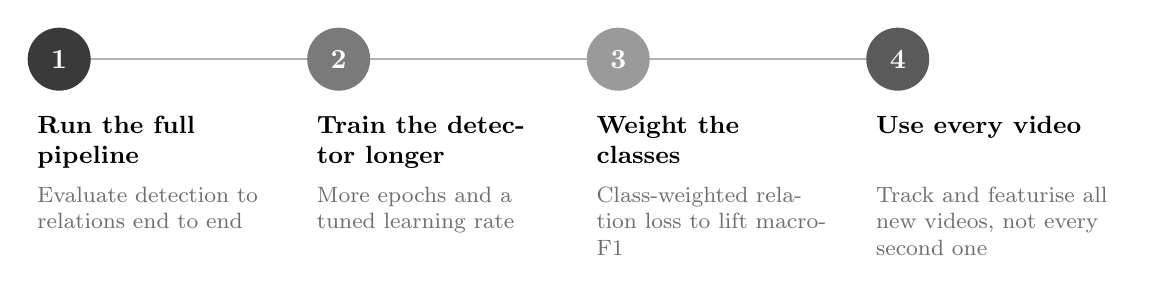
\begin{tikzpicture}
    \draw[gray!60,thick] (0.4,0) -- (11.05,0);
    \foreach \x/\c/\t/\d [count=\i] in {0.4/amber/{Run the full pipeline}/{Evaluate detection to relations end to end},
                                      3.95/teal/{Train the detector longer}/{More epochs and a tuned learning rate},
                                      7.5/peri/{Weight the classes}/{Class-weighted relation loss to lift macro-F1},
                                      11.05/coral/{Use every video}/{Track and featurise all new videos, not every second one}}{
      \node[circle,fill=\c,text=white,font=\bfseries,minimum size=0.8cm] at (\x,0) {\i};
      \node[anchor=north west,text width=3.0cm,font=\small\bfseries,align=left] at (\x-0.4,-0.6) {\t};
      \node[anchor=north west,text width=3.0cm,font=\footnotesize,text=mute,align=left] at (\x-0.4,-1.5) {\d};}
  \end{tikzpicture}
  \end{center}
  \vspace{6pt}
  {\Large\bfseries\color{amber} Thank you}
\end{frame}

\end{document}
